In der hochaufgelösten Resonanzionisationsspektroskopie ist es
sehr wichtig, über längere Messzeiten möglichst konstante Rahmenbedingungen für
die Messungen zu schaffen. Die Reproduzierbarkeit von Messungen ist nur
gewährleistet, wenn die experimentellen Parameter konstant bleiben. Der
entscheidende Parametersatz des Experiments wird durch die Lasereigenschaften
bestimmt. Für eine stabile Laserfrequenz ist das Verhalten des Laserresonators
ausschlaggebend. Temperaturschwankungen, die Dichtefluktuationen in der Luft und
im Verstärkungsmedium hervorrufen (Brechungsindexänderungen), sind ebenso wie
Vibrationen für Frequenzinstabilitäten verantwortlich. Schon bei Schwankungen
oder Drifts von wenigen MHz kann es bei schmalbandigen atomaren Übergängen zu
erheblichen Fluktuationen in der Ionisationsrate kommen. Daher ist eine aktive
Frequenzstabilisierung der verwendeten Laser unerlässlich.\par
In diesem Kapitel sollen zunächst der Vollständigkeit halber bewährte
Frequenzstabilisierungstechniken wie die Ansätze von \textit{Hänsch-Couillaud}
(Abschn. \ref{sec:haensch-couillaud}) oder \textit{Pound-Drever-Hall} (Abschn.
\ref{sec:pound-drever-hall}) kurz vorgestellt
(\cite{noertershaeuser:physik_des_lasers}) und anschließend gezielt auf das
in diesem Projekt verwendete \textit{Fringe-Offset-Locking} (Abschn.
\ref{sec:fringe-offset-locking}) eingegangen werden. Darüber hinaus
besteht auch die Anforderung, zwischen den Anregungsfrequenzen verschiedener
Isotope möglichst schnell wechseln zu können. Dies ist allein mit der
Fringe-Offset-Locking-Technik nur bedingt gegeben. Deshalb wurde diese Technik
mit einer kommerziellen Stabilisierungstechnik kombiniert, auf die am Ende
dieses Kapitals eingegangen wird.\par
Um einen Laser auf einer Frequenz zu fixieren, benötigt
man eine Referenzfrequenz. Diese kann von einem passiven, stabilen Resonator,
einem atomaren bzw. molekularen Übergang oder einem absolut stabilen Laser wie z.B.
ein Helium-Neon-Laser (He:Ne-Laser) geliefert werden.
Aus der Abweichung der Frequenz des zu stabilisierenden Lasers $\nu_{Ist}$ zur
Sollfrequenz $\nu_{Soll}$ muss ein Fehlersignal
\begin{equation}\label{eq:servoschleife_fehlersignal}
	S\approx C\cdot(\nu_{Ist}-\nu_{Soll})=C\cdot\delta\nu
\end{equation}
erzeugt werden, das hier exemplarisch linear zur Frequenzdifferenz $\delta\nu$
ist. Dieses Fehlersignal dient als Eingangssignal für eine Regelschleife, die
die Frequenz des Lasers bei Abweichung auf die Sollfrequenz zurückführt. Auf
Details der Regelschleife soll später genauer eingegangen werden (siehe
Abschn. \ref{sec:regeltechnik}). Die Generierung des Fehlersignals kann auf
verschiedene Arten geschehen, wie im Folgenden erläutert wird.

\section{Hänsch-Couillaud}\label{sec:haensch-couillaud}
\begin{figure}[h]
 	\centering
 	\fbox{\parbox{\dimexpr \linewidth - 2\fboxrule - 2\fboxsep}{
 	\centering
	    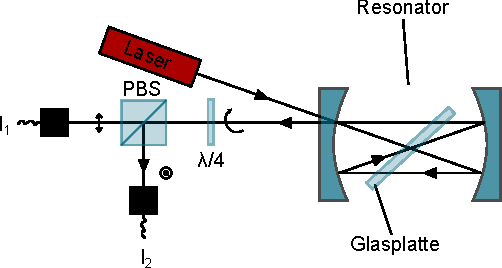
\includegraphics[width=\textwidth-4cm]{gfx/haensch-couillaud_aufbau}
	}}
	\caption[Hänsch-Couillaud-Stabilisierung - Aufbau]{Aufbau
	einer Frequenzstabilisierung nach Hänsch
	und Couillaud. Erklärungen im
	Text.}
	\label{fig:haensch-couillaud_aufbau}
\end{figure}
Die Frequenzstabilisierung nach Hänsch und Couillaud (HC)
basiert auf der \textit{Polarisationsspektroskopie}. Mithilfe eines
optischen Elements in einem festen Resonator als Referenz können verschiedene
Polarisationen des Laserlichts verschiedene Verluste erfahren. Dies lässt sich
mit einem doppelbrechenden Kristall oder einer Glasplatte im Brewsterwinkel
realisieren. Man kann das elektrische Feld des linear polarisierten einfallenden
Lichts $E_0$ in Komponenten senkrecht und parallel zur Polarisationsrichtung
zerlegen, in der das Licht minimalen Verlusten im Resonator erfährt:
\begin{equation}\label{eq:haensch-couillaud_01}
	\begin{split}
		E_{\perp}^{(0)} & = E_0\cdot\cos{(\Theta)}\\
		E_{\parallel}^{(0)} & = E_0\cdot\sin{(\Theta)}\,.
	\end{split}
\end{equation}
Dabei ist $\Theta$ der Winkel zwischen einfallender Polarisation und
Polarisation mit maximalen bzw. minimalen Verlusten. $E_{\perp}^{(0)}$ wird also
im Wesentlichen vom Einkoppelspiegel reflektiert. $E_{\parallel}^{(0)}$
wird hingegen in den Resonator eingekoppelt und erfärt bei Austritt im Falle von
Nicht-Resonanz im Resonator eine Phasenverschiebung $\delta$ zu $E_{\perp}^{(0)}$. Im Resonanzfall ist diese Phasenverschiebung null. Durch Kenntnis der Phasenverschiebung kann also eine Aussage über die Verstimmung zur Resonanz getroffen werden. Die
Komponenten des reflektierten Lichts
\begin{equation}\label{eq:haensch-couillaud_02}
	\begin{split}
		E_{\perp}^{(r)} & = E_{\perp}^{(0)}\cdot r_1\\
		E_{\parallel}^{(r)} & = E_{\parallel}^{(0)}\cdot\left(r_1-\frac{t_1^2r\mathrm{e}^{-\mathrm{i}\delta}}{r_1\left(1-r\mathrm{e}^{-\mathrm{i}\delta}\right)}\right)
	\end{split}
\end{equation}
ergeben zusammen elliptisch polarisiertes Licht und somit eine Überlagerung von
$\sigma^+$- und $\sigma^-$-Licht mit unterschiedlichen Amplituden. Dabei sind
$r_1$ und $t_1$ Reflexions- und Transmissionskoeffizienten des
Einkoppelspiegels. $r$ beschreibt die Verluste durch die Umläufe im Resonator.
Bei Phasenverschiebung überwiegt entweder der $\sigma^+$-Anteil oder der
$\sigma^-$-Anteil je nach Verstimmungsrichtung der Laserfrequenz.
Bei Resonanz sind beide Anteile gleich und es entsteht wieder linear polarisiertes Licht. Eine $\nicefrac{\lambda}{4}$-Platte erzeugt aus beiden zirkularen Anteilen ($\sigma^+$ und $\sigma^-$) lineare Anteile, welche durch einen Polarisationsstrahlteiler getrennt und letzendlich durch Photodioden
detektiert werden können. Abbildung \ref{fig:haensch-couillaud_aufbau} zeigt den
optischen Aufbau. Die Differenz der zu den Feldstärken der elektrischen Komponente
des Lichts proportionalen Ströme der Photodioden
\begin{equation}\label{eq:haensch-couillaud_fehlersignal}
	(I_1-I_2)\propto\abs{E^{(0)}}^2\cos{(\Theta)}\sin{(\Theta)}\frac{t_1^2r^2\sin{(\delta)}}{(1-r^2)+4r^2\sin^2{\left(\frac{\delta}{2}\right)}}
\end{equation}
liefert das in Abb. \ref{fig:haensch-couillaud_fehlersignal} gezeichnete
Fehlersignal mit Nulldurchgang bei den Resonanzen $\delta=2\pi n$, wobei der
schwarze Kasten den Fangbereich der Regelung markiert. Die Regelschleife muss
also auf diesen Nulldurchgang regeln.
\begin{figure}[h]
	\centering
	\footnotesize
	% GNUPLOT: LaTeX picture with Postscript
\begingroup
  \makeatletter
  \providecommand\color[2][]{%
    \GenericError{(gnuplot) \space\space\space\@spaces}{%
      Package color not loaded in conjunction with
      terminal option `colourtext'%
    }{See the gnuplot documentation for explanation.%
    }{Either use 'blacktext' in gnuplot or load the package
      color.sty in LaTeX.}%
    \renewcommand\color[2][]{}%
  }%
  \providecommand\includegraphics[2][]{%
    \GenericError{(gnuplot) \space\space\space\@spaces}{%
      Package graphicx or graphics not loaded%
    }{See the gnuplot documentation for explanation.%
    }{The gnuplot epslatex terminal needs graphicx.sty or graphics.sty.}%
    \renewcommand\includegraphics[2][]{}%
  }%
  \providecommand\rotatebox[2]{#2}%
  \@ifundefined{ifGPcolor}{%
    \newif\ifGPcolor
    \GPcolortrue
  }{}%
  \@ifundefined{ifGPblacktext}{%
    \newif\ifGPblacktext
    \GPblacktexttrue
  }{}%
  % define a \g@addto@macro without @ in the name:
  \let\gplgaddtomacro\g@addto@macro
  % define empty templates for all commands taking text:
  \gdef\gplbacktext{}%
  \gdef\gplfronttext{}%
  \makeatother
  \ifGPblacktext
    % no textcolor at all
    \def\colorrgb#1{}%
    \def\colorgray#1{}%
  \else
    % gray or color?
    \ifGPcolor
      \def\colorrgb#1{\color[rgb]{#1}}%
      \def\colorgray#1{\color[gray]{#1}}%
      \expandafter\def\csname LTw\endcsname{\color{white}}%
      \expandafter\def\csname LTb\endcsname{\color{black}}%
      \expandafter\def\csname LTa\endcsname{\color{black}}%
      \expandafter\def\csname LT0\endcsname{\color[rgb]{1,0,0}}%
      \expandafter\def\csname LT1\endcsname{\color[rgb]{0,1,0}}%
      \expandafter\def\csname LT2\endcsname{\color[rgb]{0,0,1}}%
      \expandafter\def\csname LT3\endcsname{\color[rgb]{1,0,1}}%
      \expandafter\def\csname LT4\endcsname{\color[rgb]{0,1,1}}%
      \expandafter\def\csname LT5\endcsname{\color[rgb]{1,1,0}}%
      \expandafter\def\csname LT6\endcsname{\color[rgb]{0,0,0}}%
      \expandafter\def\csname LT7\endcsname{\color[rgb]{1,0.3,0}}%
      \expandafter\def\csname LT8\endcsname{\color[rgb]{0.5,0.5,0.5}}%
    \else
      % gray
      \def\colorrgb#1{\color{black}}%
      \def\colorgray#1{\color[gray]{#1}}%
      \expandafter\def\csname LTw\endcsname{\color{white}}%
      \expandafter\def\csname LTb\endcsname{\color{black}}%
      \expandafter\def\csname LTa\endcsname{\color{black}}%
      \expandafter\def\csname LT0\endcsname{\color{black}}%
      \expandafter\def\csname LT1\endcsname{\color{black}}%
      \expandafter\def\csname LT2\endcsname{\color{black}}%
      \expandafter\def\csname LT3\endcsname{\color{black}}%
      \expandafter\def\csname LT4\endcsname{\color{black}}%
      \expandafter\def\csname LT5\endcsname{\color{black}}%
      \expandafter\def\csname LT6\endcsname{\color{black}}%
      \expandafter\def\csname LT7\endcsname{\color{black}}%
      \expandafter\def\csname LT8\endcsname{\color{black}}%
    \fi
  \fi
  \setlength{\unitlength}{0.0500bp}%
  \begin{picture}(7200.00,5040.00)%
    \gplgaddtomacro\gplbacktext{%
      \csname LTb\endcsname%
      \put(860,1120){\makebox(0,0)[r]{\strut{}-1}}%
      \put(860,1920){\makebox(0,0)[r]{\strut{}-0.5}}%
      \put(860,2719){\makebox(0,0)[r]{\strut{} 0}}%
      \put(860,3519){\makebox(0,0)[r]{\strut{} 0.5}}%
      \put(860,4319){\makebox(0,0)[r]{\strut{} 1}}%
      \put(980,440){\makebox(0,0){\strut{}-3}}%
      \put(1957,440){\makebox(0,0){\strut{}-2}}%
      \put(2933,440){\makebox(0,0){\strut{}-1}}%
      \put(3910,440){\makebox(0,0){\strut{} 0}}%
      \put(4886,440){\makebox(0,0){\strut{} 1}}%
      \put(5863,440){\makebox(0,0){\strut{} 2}}%
      \put(6839,440){\makebox(0,0){\strut{} 3}}%
      \put(160,2719){\rotatebox{-270}{\makebox(0,0){\strut{}Amplitude}}}%
      \put(3909,140){\makebox(0,0){\strut{}Phasenverschiebung relativ zur Resonanz $\nicefrac{\delta}{\pi}$}}%
    }%
    \gplgaddtomacro\gplfronttext{%
    }%
    \gplbacktext
    \put(0,0){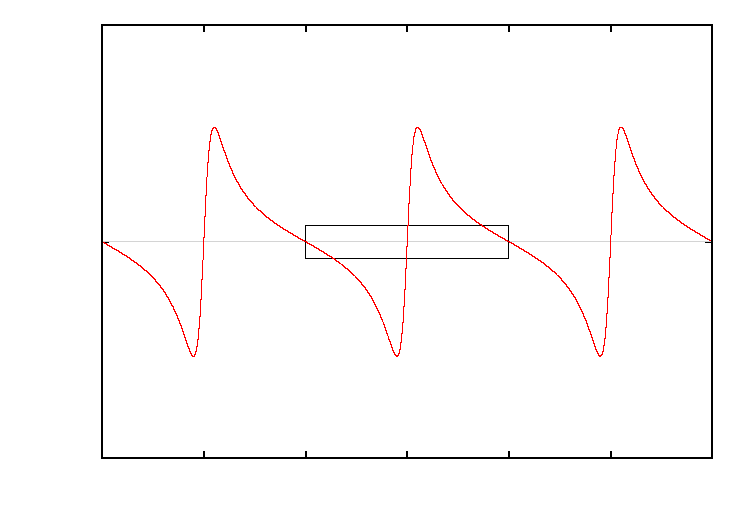
\includegraphics{haensch-couillaud_fehlersignal}}%
    \gplfronttext
  \end{picture}%
\endgroup

	\caption[Hänsch-Couillaud-Stabilisierung - Fehlersignal]{Phasenabhängige
	Fehlersignal der Hänsch-Couillaud-Stabilisierung gemäß Gl. \eqref{eq:haensch-couillaud_fehlersignal}.
	Der markierte Bereich ist der
	Fangbereich der Regelung.}
	\label{fig:haensch-couillaud_fehlersignal}
\end{figure}

\section{Pound-Drever-Hall}\label{sec:pound-drever-hall}
\begin{figure}[h]
 	\centering
 	\fbox{\parbox{\dimexpr \linewidth - 2\fboxrule - 2\fboxsep}{
 	\centering
	    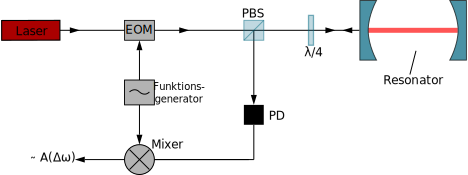
\includegraphics[width=\textwidth-0.5cm]{gfx/pound-drever-hall_aufbau}
	}}
	\caption[Pound-Drever-Hall-Stabilisierung - Aufbau]{Aufbau
	einer Frequenzstabilisierung nach Pound, Drever und Hall. Erklärungen dazu
	finden sich im Text.}
	\label{fig:pound-drever-hall_aufbau}
\end{figure}
Ein Aufbau des Verfahrens nach Pound, Drever und Hall (PDH) ist in Abb.
\ref{fig:pound-drever-hall_aufbau} dargestellt.
Das Laserlicht mit der Frequenz $\omega_L$ wird mittels eines \textit{elektrooptischen Modulators}, kurz EOM, in der Phase gemäß
\begin{equation}\label{eq:pound-drever-hall_01}
	E=\E_0\cos{\left(\omega_Lt+\delta\cos{(\omega_mt)}\right)}
\end{equation}
mit einem kleinen Modulationsindex $\delta\ll1$ moduliert. Dabei treten in
erster Ordnung gegenphasige Seitenbänder mit der Frequenz $\omega_L\pm\omega_m$
auf. Als Referenz dient wieder wie oben ein Resonator, in den bei Resonanz ein
Teil des Trägerlichts eingekoppelt wird. Die Seitenbänder und der restliche Teil
des Trägers werden reflektiert. Da das Licht im Resonator bei Resonanz einen
Phasensprung von $\pi$ erfährt, ergibt sich für die Nettoleistung des
reflektierten Trägerlichts eine Abschwächung durch destruktive Interferenz.
Da die beiden Seitenbänder gegenphasig schwingen, haben die Schwebungen dieser
Seitenbänder mit dem Träger unterschiedliche Vorzeichen. Im Resonanzfall heben
sich also die Schwebungssignale aufgrund gleicher Amplitude gegenseitig auf, was
vollständige destruktive Interferenz des Fehlersignals bedeutet. Bei geringer
Verstimmung der Laserfrequenz zur Resonanzfrequenz des Resonators ist die
Phasenverschiebung im Resonator nicht mehr $\pi$, was zu unterschiedlichen Amplituden der
Schwebungssignale führt. Das resultierende Signal ist also von null
verschieden.\par
Die Trennung des einfallenden Lichts vom zu analysierenden Licht kann mit einer
$\nicefrac{\lambda}{4}$-Platte und einem Polarisationsstrahlteiler realisiert
werden. Für den Photodiodenstrom erhält man in Abhängigkeit von der Verstimmung
des Trägerlichts zur Resonanz
\begin{equation}\label{eq:pound-drever-hall_fehlersignal}
	I(\Delta\omega,\omega_m)\propto
	J_0(\delta)J_1(\delta)\left[A(\Delta\omega)\cos{(\omega_mt)}+D(\Delta\omega)\sin{(\omega_mt)}\right]\,,
\end{equation}
wobei $J_{0,1}$ nullte und erste Ordnung von Besselfunktionen sind. Mischt man
das Signal mit dem der Modulation, erhält man als Ausgangssignal den zur
Modulation gleichphasigen Anteil von
Gl. \eqref{eq:pound-drever-hall_fehlersignal}, der proportional zu
$A(\Delta\omega)$ ist.
Abbildung \ref{fig:pound-drever-hall_fehlersignal} zeigt die Abhängigkeit dieses
Fehlsignals zur Verstimmung $\Delta\omega$. Um den Laser auf Resonanz zu halten,
muss auf den Nulldurchgang geregelt werden.
\begin{figure}[h]
	\centering
	\footnotesize
	% GNUPLOT: LaTeX picture with Postscript
\begingroup
  \makeatletter
  \providecommand\color[2][]{%
    \GenericError{(gnuplot) \space\space\space\@spaces}{%
      Package color not loaded in conjunction with
      terminal option `colourtext'%
    }{See the gnuplot documentation for explanation.%
    }{Either use 'blacktext' in gnuplot or load the package
      color.sty in LaTeX.}%
    \renewcommand\color[2][]{}%
  }%
  \providecommand\includegraphics[2][]{%
    \GenericError{(gnuplot) \space\space\space\@spaces}{%
      Package graphicx or graphics not loaded%
    }{See the gnuplot documentation for explanation.%
    }{The gnuplot epslatex terminal needs graphicx.sty or graphics.sty.}%
    \renewcommand\includegraphics[2][]{}%
  }%
  \providecommand\rotatebox[2]{#2}%
  \@ifundefined{ifGPcolor}{%
    \newif\ifGPcolor
    \GPcolortrue
  }{}%
  \@ifundefined{ifGPblacktext}{%
    \newif\ifGPblacktext
    \GPblacktexttrue
  }{}%
  % define a \g@addto@macro without @ in the name:
  \let\gplgaddtomacro\g@addto@macro
  % define empty templates for all commands taking text:
  \gdef\gplbacktext{}%
  \gdef\gplfronttext{}%
  \makeatother
  \ifGPblacktext
    % no textcolor at all
    \def\colorrgb#1{}%
    \def\colorgray#1{}%
  \else
    % gray or color?
    \ifGPcolor
      \def\colorrgb#1{\color[rgb]{#1}}%
      \def\colorgray#1{\color[gray]{#1}}%
      \expandafter\def\csname LTw\endcsname{\color{white}}%
      \expandafter\def\csname LTb\endcsname{\color{black}}%
      \expandafter\def\csname LTa\endcsname{\color{black}}%
      \expandafter\def\csname LT0\endcsname{\color[rgb]{1,0,0}}%
      \expandafter\def\csname LT1\endcsname{\color[rgb]{0,1,0}}%
      \expandafter\def\csname LT2\endcsname{\color[rgb]{0,0,1}}%
      \expandafter\def\csname LT3\endcsname{\color[rgb]{1,0,1}}%
      \expandafter\def\csname LT4\endcsname{\color[rgb]{0,1,1}}%
      \expandafter\def\csname LT5\endcsname{\color[rgb]{1,1,0}}%
      \expandafter\def\csname LT6\endcsname{\color[rgb]{0,0,0}}%
      \expandafter\def\csname LT7\endcsname{\color[rgb]{1,0.3,0}}%
      \expandafter\def\csname LT8\endcsname{\color[rgb]{0.5,0.5,0.5}}%
    \else
      % gray
      \def\colorrgb#1{\color{black}}%
      \def\colorgray#1{\color[gray]{#1}}%
      \expandafter\def\csname LTw\endcsname{\color{white}}%
      \expandafter\def\csname LTb\endcsname{\color{black}}%
      \expandafter\def\csname LTa\endcsname{\color{black}}%
      \expandafter\def\csname LT0\endcsname{\color{black}}%
      \expandafter\def\csname LT1\endcsname{\color{black}}%
      \expandafter\def\csname LT2\endcsname{\color{black}}%
      \expandafter\def\csname LT3\endcsname{\color{black}}%
      \expandafter\def\csname LT4\endcsname{\color{black}}%
      \expandafter\def\csname LT5\endcsname{\color{black}}%
      \expandafter\def\csname LT6\endcsname{\color{black}}%
      \expandafter\def\csname LT7\endcsname{\color{black}}%
      \expandafter\def\csname LT8\endcsname{\color{black}}%
    \fi
  \fi
  \setlength{\unitlength}{0.0500bp}%
  \begin{picture}(7200.00,5040.00)%
    \gplgaddtomacro\gplbacktext{%
      \csname LTb\endcsname%
      \put(860,1056){\makebox(0,0)[r]{\strut{}-0.4}}%
      \put(860,1888){\makebox(0,0)[r]{\strut{}-0.2}}%
      \put(860,2719){\makebox(0,0)[r]{\strut{} 0}}%
      \put(860,3551){\makebox(0,0)[r]{\strut{} 0.2}}%
      \put(860,4383){\makebox(0,0)[r]{\strut{} 0.4}}%
      \put(980,440){\makebox(0,0){\strut{}-10}}%
      \put(2445,440){\makebox(0,0){\strut{}-5}}%
      \put(3909,440){\makebox(0,0){\strut{} 0}}%
      \put(5374,440){\makebox(0,0){\strut{} 5}}%
      \put(6839,440){\makebox(0,0){\strut{} 10}}%
      \put(160,2719){\rotatebox{-270}{\makebox(0,0){\strut{}$A(\Delta\omega)$}}}%
      \put(3909,140){\makebox(0,0){\strut{}Verstimmung zur Resonanz $\Delta\omega$}}%
    }%
    \gplgaddtomacro\gplfronttext{%
    }%
    \gplbacktext
    \put(0,0){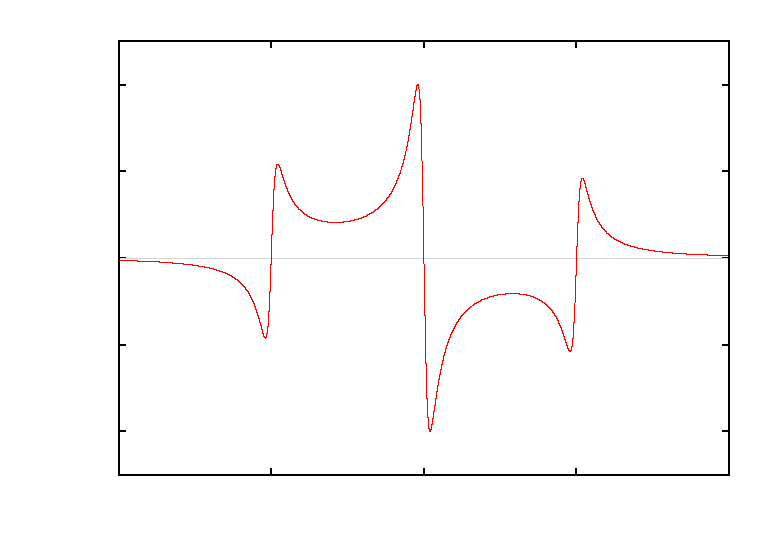
\includegraphics{pound-drever-hall_fehlersignal}}%
    \gplfronttext
  \end{picture}%
\endgroup

	\caption[Hänsch-Couillaud-Stabilisierung - Fehlersignal]{Fehlersignal der
	Pound-Drever-Hall-Stabilisierung gemäß Gl. 
	\eqref{eq:pound-drever-hall_fehlersignal}. Die Modulation $\pm\omega_m$ liegt
	bei $\pm5$.}
	\label{fig:pound-drever-hall_fehlersignal}
\end{figure}

\section{Fringe-Offset-Locking}\label{sec:fringe-offset-locking}
Die oben erklärten Techniken sind darauf ausgelegt einen einzigen Laser zu
stabilisieren. Ein Frequenzscan ist bei der PDH-Methode nur sehr eingeschränkt
möglich. Der Referenz-Resonator müsste sehr langsam verstimmt werden, damit die
Regelung nachkommt. Größere Frequenzsprünge sind auch bei der HC-Methode
nur bedingt möglich. Im hier diskutierten Experiment wird allerdings eine
Stabilisierung benötigt, die drei Laser unabhängig voneinander kontrollieren
kann. Gleichermaßen wird schnelles Abstimmen auf eine gewünschte
Frequenzen gefordert. Aus Kosten- und Aufwandsgründen ist es dabei von Vorteil, wenn für alle drei Laser dieselbe
Referenz verwendet werden kann, ohne dass diese eine Abhängigkeit der Laser
untereinander verursacht. Eine hervorragende Methode dafür ist das
Fringe-Offset-Locking (FOL). Diese Technik soll im Folgenden genauer betrachtet
werden.

\subsection{Fabry-Perot-Interferometer}\label{subsec:fabry-perot-interferometer}
Eine entscheidende Rolle spielt hier ein sog.
\textit{Fabry-Perot-Interferometer}, kurz FPI, das sowohl
als feste Referenz als auch als Frequenzspektrum-Analysator dienen kann.
Beide Varianten sollen in diesem Abschnitt vorgestellt werden. Die Ausführungen
stützen sich auf die Arbeiten \cite{wiche:1997:diplomarbeit} und
\cite{kuschnick:2000:diplomarbeit}.

\subsubsection{Festes FPI}\label{subsubsec:festes_FPI}
Ein FPI ist ein Resonator bestehend aus zwei planparallelen oder, wie später
beschrieben, gekrümmten Spiegeln mit den Reflektivitäten $R_1$ und $R_2$ und dem
Abstand $L$ wie in Abb.
\ref{fig:FPI_planparallel} schematisch dargestellt.
\begin{figure}[h]
 	\centering
 	\fbox{\parbox{\dimexpr \linewidth - 2\fboxrule - 2\fboxsep}{
 	\centering
	    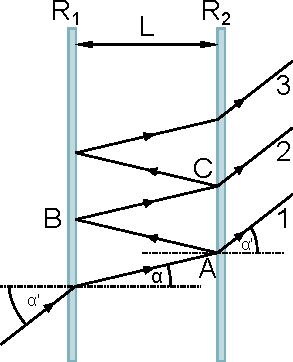
\includegraphics[width=7cm]{gfx/FPI_planparallel}
	}}
	\caption[FPI - planparallel]{Strahlengang in einem
	planprarallelen Fabry-Perot-Interferometer.}
	\label{fig:FPI_planparallel}
\end{figure}
Licht, das unter dem Winkel
$\alpha'$ von links eingestrahlt wird, wird nach dem Gesetz von Snellius
\begin{equation}\label{eq:snellius}
	\frac{n_r}{n_{ext}}=\frac{\sin{(\alpha')}}{\sin{(\alpha)}}
\end{equation}
auf den Winkel $\alpha$ gebrochen, wenn $n_r$ bzw. $n_{ext}$ der Brechungsindex
des Resonators bzw. der Raumluft ist. Für die Amplitude des elektrischen Feldes
$E_1$ des direkt transmittierten Lichts ergibt sich
\begin{equation}\label{eq:FPI_E1}
	E_1=E_0t_1t_2\mathrm{e}^{\mathrm{i}\phi'}\,.
\end{equation}
Hierbei ist $E_0$ die Amplitude des elektrischen Feldes des einfallenden Lichts,
$t_1$ und $t_2$ die Transmissionskoeffizienten für das elektrische Feld
der beiden Spiegel und $\phi'$ die Phasenänderung der elektromagnetischen Welle
nach direkter Transmission des FPIs. Für die Amplitude des elektrischen Feldes des
transmittierten Lichts nach einem Umlauf
(Eintritt$\rightarrow$A$\rightarrow$B$\rightarrow$C$\rightarrow$Austritt) gilt
\begin{equation}\label{eq:FPI_E2}
	\begin{split}
		E_2
		&=E_0t_1r_2r_1t_2\mathrm{e}^{\mathrm{i}\phi'}\mathrm{e}^{\mathrm{i}2\phi}\\
		&=E_1r_1r_2\mathrm{e}^{\mathrm{i}2\phi}\,.
	\end{split}
\end{equation}
$2\phi$ ist hier die Phasenverschiebung, die das Licht nach einem Umlauf im
Resonator (A$\rightarrow$B$\rightarrow$C) erhält. Allgemein gilt für den m-ten
transmittierten Strahl
\begin{equation}\label{eq:FPI_Em}
	E_m=E_1(r_1r_2)^m\mathrm{e}^{\mathrm{i}m2\phi}\,.
\end{equation}
Die Phasenverschiebung $2\phi=kL_{opt}$ ist abhängig von der optischen Weglänge
$L_{opt}=\overline{AB}+\overline{BC}=\frac{2n_rL}{\cos{(\alpha)}}$ und der Wellenzahl des
Lichts $k=2\pi\frac{\nu}{c}$. Somit ergibt sich also
\begin{equation}\label{eq:FPI_phase}
	\phi=\frac{2\pi n_r\nu L}{\cos{(\alpha)}c}\,.
\end{equation}
Das gesamte elektrische Feld des transmittierten Lichts ist eine Superposition
aller transmittierter Einzelfelder:
\begin{equation}\label{eq:FPI_Et}
	\begin{split}
		E_t
		&=E_1\cdot\sum\limits_{m=0}^\infty(r_1r_2)^m\mathrm{e}^{\mathrm{i}2m\phi}\\
		&=E_1\frac{1}{1-r_1r_2\mathrm{e}^{\mathrm{i}2\phi}}\,.
	\end{split}
\end{equation}
Die Auflösung der Summe folgt gemäß der geometrischen Reihe
\begin{equation}\label{eq:geometrsiche_summe}
	\begin{split}
		\sum_{k=0}^{\infty}q^k &=\lim_{n\to\infty}\sum_{k=0}^{n}q^k\\
		&=\lim_{n\to\infty}\frac{1-q^{n+1}}{1-q}\\
		&=\frac{1}{1-q}\\
		&\text{mit}\\
		q&=r_1r_2\mathrm{e}^{\mathrm{i}2\phi}<1\,.
	\end{split}
\end{equation}
Mit
\begin{equation}\label{eq:betrags-quadrat_imag}
	\begin{split}
		\abs{1-r_1r_2\mathrm{e}^{\mathrm{i}2\phi}}^2&=\abs{1-r_1r_2\cos(2\phi)-\mathrm{i}r_1r_2\sin{(2\phi})}^2\\
		&=\left[1-r_1r_2\cos(2\phi)\right]^2+r_1^2r_2^2\sin^2{(2\phi)}\\
		&=1-2r_1r_2\cos{(2\phi)}+r_1^2r_2^2
	\end{split}
\end{equation}
und Gl. \eqref{eq:FPI_E1} folgt für die gesamte transmittierte Leistung
\begin{equation}\label{eq:FPI_transmission}
	\begin{split}
		T=\frac{\abs{E_t}^2}{\abs{E_0}^2}
		&=\frac{t_1^2t_2^2}{1-2r_1r_2\cos{(2\phi)}+r_1^2r_2^2}\\
		&=\frac{(1-R_1)(1-R_2)}{\left(1-\sqrt{R_1R_2}\right)^2+4\sqrt{R_1R_2}\sin^2{(\phi)}}\\
		&\text{mit}\quad
		R_i=r_i^2
		\quad\text{und}\quad
		t_i^2=1-r_i^2=1-R_i\,,
	\end{split}
\end{equation}
wobei im letzten Schritt Additionstheoreme angewendet wurden.
Setzt man nun gleiche Reflektivitäten der beiden Spiegel $R_1=R_2=R$ voraus und
substituiert $\kappa:=\frac{4R}{(1-R)^2}$ erhält man eine sog.
\textit{Airy-Funktion}
\begin{equation}\label{eq:FPI_airy-funktion}
	T=\frac{1}{1+\kappa\sin^2{(\phi)}}\,.
\end{equation}
Wie leicht zu erkennen ist, ist die Transmissionsfunktion $\pi$-periodisch in
der Phase $\phi$ und gleichzeitig in der Frequenz des Lasers, da die Phase nach
Gl. \eqref{eq:FPI_phase} frequenzabhängig ist. Abbildung
\ref{fig:airy-funktion} zeigt die Airy-Funktion für verschiedene Finessen
$F$ bzw. Reflektivitäten der Spiegel.
\begin{figure}[h]
	\centering
	\footnotesize
	% GNUPLOT: LaTeX picture with Postscript
\begingroup
  \makeatletter
  \providecommand\color[2][]{%
    \GenericError{(gnuplot) \space\space\space\@spaces}{%
      Package color not loaded in conjunction with
      terminal option `colourtext'%
    }{See the gnuplot documentation for explanation.%
    }{Either use 'blacktext' in gnuplot or load the package
      color.sty in LaTeX.}%
    \renewcommand\color[2][]{}%
  }%
  \providecommand\includegraphics[2][]{%
    \GenericError{(gnuplot) \space\space\space\@spaces}{%
      Package graphicx or graphics not loaded%
    }{See the gnuplot documentation for explanation.%
    }{The gnuplot epslatex terminal needs graphicx.sty or graphics.sty.}%
    \renewcommand\includegraphics[2][]{}%
  }%
  \providecommand\rotatebox[2]{#2}%
  \@ifundefined{ifGPcolor}{%
    \newif\ifGPcolor
    \GPcolortrue
  }{}%
  \@ifundefined{ifGPblacktext}{%
    \newif\ifGPblacktext
    \GPblacktexttrue
  }{}%
  % define a \g@addto@macro without @ in the name:
  \let\gplgaddtomacro\g@addto@macro
  % define empty templates for all commands taking text:
  \gdef\gplbacktext{}%
  \gdef\gplfronttext{}%
  \makeatother
  \ifGPblacktext
    % no textcolor at all
    \def\colorrgb#1{}%
    \def\colorgray#1{}%
  \else
    % gray or color?
    \ifGPcolor
      \def\colorrgb#1{\color[rgb]{#1}}%
      \def\colorgray#1{\color[gray]{#1}}%
      \expandafter\def\csname LTw\endcsname{\color{white}}%
      \expandafter\def\csname LTb\endcsname{\color{black}}%
      \expandafter\def\csname LTa\endcsname{\color{black}}%
      \expandafter\def\csname LT0\endcsname{\color[rgb]{1,0,0}}%
      \expandafter\def\csname LT1\endcsname{\color[rgb]{0,1,0}}%
      \expandafter\def\csname LT2\endcsname{\color[rgb]{0,0,1}}%
      \expandafter\def\csname LT3\endcsname{\color[rgb]{1,0,1}}%
      \expandafter\def\csname LT4\endcsname{\color[rgb]{0,1,1}}%
      \expandafter\def\csname LT5\endcsname{\color[rgb]{1,1,0}}%
      \expandafter\def\csname LT6\endcsname{\color[rgb]{0,0,0}}%
      \expandafter\def\csname LT7\endcsname{\color[rgb]{1,0.3,0}}%
      \expandafter\def\csname LT8\endcsname{\color[rgb]{0.5,0.5,0.5}}%
    \else
      % gray
      \def\colorrgb#1{\color{black}}%
      \def\colorgray#1{\color[gray]{#1}}%
      \expandafter\def\csname LTw\endcsname{\color{white}}%
      \expandafter\def\csname LTb\endcsname{\color{black}}%
      \expandafter\def\csname LTa\endcsname{\color{black}}%
      \expandafter\def\csname LT0\endcsname{\color{black}}%
      \expandafter\def\csname LT1\endcsname{\color{black}}%
      \expandafter\def\csname LT2\endcsname{\color{black}}%
      \expandafter\def\csname LT3\endcsname{\color{black}}%
      \expandafter\def\csname LT4\endcsname{\color{black}}%
      \expandafter\def\csname LT5\endcsname{\color{black}}%
      \expandafter\def\csname LT6\endcsname{\color{black}}%
      \expandafter\def\csname LT7\endcsname{\color{black}}%
      \expandafter\def\csname LT8\endcsname{\color{black}}%
    \fi
  \fi
  \setlength{\unitlength}{0.0500bp}%
  \begin{picture}(7200.00,5040.00)%
    \gplgaddtomacro\gplbacktext{%
      \csname LTb\endcsname%
      \put(540,830){\makebox(0,0)[r]{\strut{}0}}%
      \put(540,1780){\makebox(0,0)[r]{\strut{}0.5}}%
      \put(540,2729){\makebox(0,0)[r]{\strut{}1}}%
      \put(1023,440){\makebox(0,0){\strut{} 0}}%
      \put(1932,440){\makebox(0,0){\strut{} 0.5}}%
      \put(2841,440){\makebox(0,0){\strut{} 1}}%
      \put(3749,440){\makebox(0,0){\strut{} 1.5}}%
      \put(4658,440){\makebox(0,0){\strut{} 2}}%
      \put(5567,440){\makebox(0,0){\strut{} 2.5}}%
      \put(6476,440){\makebox(0,0){\strut{} 3}}%
      \put(1023,4639){\makebox(0,0){\strut{}0}}%
      \put(2841,4639){\makebox(0,0){\strut{}300}}%
      \put(4658,4639){\makebox(0,0){\strut{}600}}%
      \put(6476,4639){\makebox(0,0){\strut{}900}}%
      \put(200,1739){\rotatebox{-270}{\makebox(0,0){\strut{}Transmission}}}%
      \put(3749,140){\makebox(0,0){\strut{}Phase $\nicefrac{\phi}{\pi}$}}%
      \put(3749,4938){\makebox(0,0){\strut{}Frequenz $\nu$ [MHz]}}%
      \put(1750,2957){\makebox(0,0)[l]{\strut{}FSR}}%
    }%
    \gplgaddtomacro\gplfronttext{%
      \csname LTb\endcsname%
      \put(1620,4226){\makebox(0,0)[r]{\strut{}$F=2$}}%
      \csname LTb\endcsname%
      \put(1620,3926){\makebox(0,0)[r]{\strut{}$F=10$}}%
      \csname LTb\endcsname%
      \put(1620,3626){\makebox(0,0)[r]{\strut{}$F=100$}}%
    }%
    \gplgaddtomacro\gplbacktext{%
      \csname LTb\endcsname%
      \put(3756,3368){\makebox(0,0)[r]{\strut{} 0}}%
      \put(3756,3677){\makebox(0,0)[r]{\strut{} 50}}%
      \put(3756,3986){\makebox(0,0)[r]{\strut{} 100}}%
      \put(3756,4295){\makebox(0,0)[r]{\strut{} 150}}%
      \put(3876,2921){\makebox(0,0){\strut{} 0}}%
      \put(4440,2921){\makebox(0,0){\strut{} 0.2}}%
      \put(5004,2921){\makebox(0,0){\strut{} 0.4}}%
      \put(5567,2921){\makebox(0,0){\strut{} 0.6}}%
      \put(6131,2921){\makebox(0,0){\strut{} 0.8}}%
      \put(6695,2921){\makebox(0,0){\strut{} 1}}%
      \put(3356,3708){\rotatebox{-270}{\makebox(0,0){\strut{}Finesse}}}%
      \put(5285,3280){\makebox(0,0){\strut{}Reflektivit{"a}t}}%
    }%
    \gplgaddtomacro\gplfronttext{%
    }%
    \gplbacktext
    \put(0,0){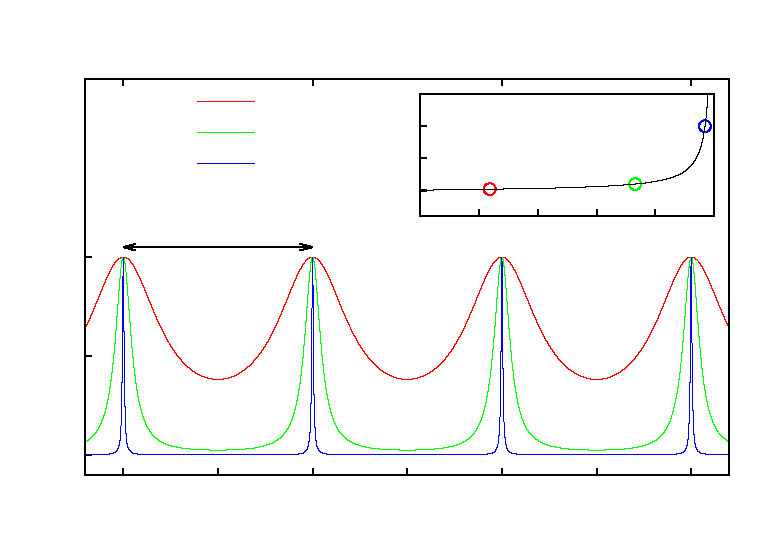
\includegraphics{airy-funktion}}%
    \gplfronttext
  \end{picture}%
\endgroup

	\caption[Airy-Funktion]{Airy-Funktion
	in Abhängigkeit von der Phase bzw.
	der Laserfrequenz. Eingezeichnet ist
	der freie Spektralbereich des
	Interferometers (exemplarisch mit $\text{FSR}=300\,$MHz). Rechts oben ist die
	Finesse in Abhängigkeit zur
	Reflektivität der Spiegel dargestellt.}
	\label{fig:airy-funktion}
\end{figure}
Bei hoher Finesse sind scharfe
äquidistante Transmissionsmaxima zu erkennen. Mit der Annahme, dass das Licht
mit dem Winkel $\alpha'\ll1$ eingestrahlt wird, haben nach Gl.
\eqref{eq:FPI_phase} die Maxima $i$ einen Abstand von
\begin{equation}\label{eq:FPI_transmissionsmaxima}
	\Delta\nu=\abs{\nu_{i+1}-\nu_i}=\frac{c}{2\pi	n_rL}(\phi_{i+1}-\phi_i)=\frac{c}{2n_rL}\,.
\end{equation}
Dieser Frequenzabstand wird als \textit{freier Spektralbereich}, kurz FSR, des
FPIs bezeichnet und kann in Abhängigkeit von der optischen Weglänge $U$ für
einen Umlauf geschrieben werden:
\begin{equation}\label{eq:FPI_FSR_01}
	\text{FSR}=\frac{c}{U}
	\quad\text{mit}\quad
	U=2n_rL\,.
\end{equation}
In Abb. \ref{fig:airy-funktion} ist der FSR exemplarisch mit $300\,$MHz
angegeben. Damit das FPI unempfindlich auf kleine Variationen des Einfallswinkels $\alpha'$
ist, wird hier im Gegensatz zu einem planparallelen ein \textit{konfokales} FPI
verwendet wie es in Abb. \ref{fig:FPI_konfokal} dargestellt ist.
\begin{figure}[h]
 	\centering
 	\fbox{\parbox{\dimexpr \linewidth - 2\fboxrule - 2\fboxsep}{
 	\centering
	    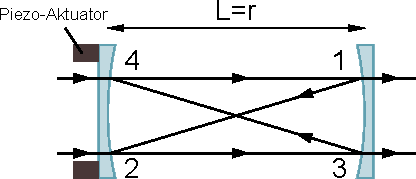
\includegraphics[width=\textwidth-4cm]{gfx/FPI_konfokal}
	}}
	\caption[FPI - konfokal]{Strahlengang in einem
	konfokalen Fabry-Perot-Interferometer. Die
	Krümmungsradien der Spiegel entsprechen dem
	Spiegelabstand. Ein ringförmiger Piezo-Aktuator dient zur
	Verstimmbarkeit des Spiegelabstands (vgl. Abschn.
	\ref{subsubsec:scanning_FPI}).}
	\label{fig:FPI_konfokal}
\end{figure}
Der Abstand $L$ ist so gewählt, dass er den Spiegelradien entspricht und sich
ein gemeinsamer Fokus in der Mitte bildet. Da das Licht
in diesem Fall zwei Umläufe ($1\rightarrow2\rightarrow3\rightarrow4$)
benötigt, damit die transmittierten Felder interferieren können,
verdoppelt sich die optische Weglänge auf $U=4n_rL$, was zu einem FSR von
\begin{equation}\label{eq:FPI_FSR_02}
	\text{FSR}=\frac{c}{4n_rL}
\end{equation}
führt. Die eben schon erwähnte Finesse ist ein Maß für die Peakbreite der
Transmissionsfunktion \eqref{eq:FPI_airy-funktion} und wichtet den FSR mit der
inversen Halbwertsbreite der Peaks:
\begin{equation}\label{eq:FPI_finesse}
	\begin{split}
		F&=\frac{\text{FSR}}{\Delta\nu_{\nicefrac{1}{2}}}\\
		&=\frac{\pi}{2\arcsin(\nicefrac{1}{\sqrt{\kappa}})}\,.
	\end{split}
\end{equation}
Die Halbwertsbreite erhält man aus Gl. \eqref{eq:FPI_airy-funktion} über
$T(\phi_{\nicefrac{1}{2}})=\nicefrac{1}{2}$ und Auflösen nach
$\phi_{\nicefrac{1}{2}}$. Nach Entwicklung in erster Ordnung lässt sich für
$R>0,5$ die Finesse näherungsweise zu
$F\approx\frac{\pi\sqrt{\kappa}}{2}=\frac{\pi\sqrt{R}}{1-R}$ berechnen.
Ebenfalls ist die Finesse - wie in Abb. \ref{fig:airy-funktion} aufgetragen - abhängig von der Reflektivität der Spiegel. Zu erkennen ist, dass hohe Finessen erst bei Reflektivitäten nahe 1 erreicht werden.

\subsubsection{Scanning FPI}\label{subsubsec:scanning_FPI}
Als fester Resonator kann das FPI dazu dienen, die
Referenzenfrequenz in Abschn. \ref{sec:haensch-couillaud} und
\ref{sec:pound-drever-hall} vorzugeben. Es ist jedoch auch möglich anstatt durch
Verstimmung der Laserfrequenz durch Variation der Resonatorlänge
Transmissionsmaxima zu erhalten. Dies ist leicht aus der linearen Abhängigkeit
der Phase $\phi$ von der Resonatorlänge $L$ in Gl. \eqref{eq:FPI_phase}
ersichtlich. Die Längenveränderung ist mit einem ringförmigen Piezo-Aktuator
realisierbar, wie in Abb. \ref{fig:FPI_konfokal} eingezeichnet. Die Ausdehnung
eines Piezo-Aktuators ist näherungsweise linear in der Ladungsmenge, die auf ihn
fließt, und somit linear bei konstantem Stromfluss. Gleichermaßen linear ist er
damit auch zur angelegten Spannung. Für ein konfokales FPI folgt für die
Längenperioden $\Delta L$ benachbarter Transmissionsmaxima mit $\phi=\pi$
\begin{equation}\label{eq:FPI_laengenperiode}
	\Delta L=\frac{c}{4n_r\nu}=\frac{\lambda}{4n_r}\,.
\end{equation}
Die Längenperiode entspricht also einem Viertel der Wellenlänge, was sofort
einsichtig ist, da die Längenänderung somit für einen Umlauf genau $\lambda$ ist
und zur konstruktiven Interferenz führt. Mit dieser Information lässt sich nun
bei zeitlich linearer Längenvariation eine Kalibration zwischen Zeit und
Frequenz durchführen
\begin{equation}\label{eq:FPI_zeit-eichung}
	\frac{\Delta T}{\Delta\nu}=\frac{\Delta T}{\Delta L}\cdot\frac{\Delta
	L}{\Delta\nu}=\frac{1}{v}\cdot\frac{-\lambda}{4n_r\text{FSR}}=\frac{-c}{4v\nu
	n_r\text{FSR}}=:\fracd{t}{\nu}\,,
\end{equation}
wobei $v$ die Geschwindigkeit ist, mit der sich der Piezo-Aktuator ausdehnt.
Das Minus folgt aus einer negativen Längenänderung des Interferometers
(Ausdehnung des Piezo-Aktuators).\par
Es ist also für das zeitliche Transmissionssignal unerheblich, ob man
Laserfrequenz oder Resonatorlänge variiert. Die Längenvariation birgt den großen
Vorteil, dass man das Verhalten mehrerer Laser gleichzeitig überwachen kann,
sofern man eine weitere Referenz wie z.B. einen frequenzstabilen He:Ne-Laser
verwendet.
Dabei müssen alle Laserstrahlen auf gleichem Weg das FPI durchlaufen und
danach ihr Transmissionsverhalten getrennt detektiert werden. Dabei wird
die Länge des Interferometers mit einer
Sägezahnspannung periodisch linear durchgefahren. Wie genau
diese Laserkontrolle realisiert wird, soll im folgenden Abschnitt näher erklärt werden.

\subsection{Relativfrequenzberechnung
und Laserkontrolle}\label{subsec:relativfrequenzberechnung_und_laserkontrolle}
In diesem Abschnitt wird das Funktionsprinzip des FOL anhand
eines zu stabilisierenden Lasers und eines Referenzlasers beschrieben. Die
konkrete Realisierung soll in Abschn. \ref{sec:elektronik_laserkontrolle}
detailliert vorgestellt werden.\par
\begin{figure}[h]
 	\centering
 	\fbox{\parbox{\dimexpr \linewidth - 2\fboxrule - 2\fboxsep}{
 	\centering
	    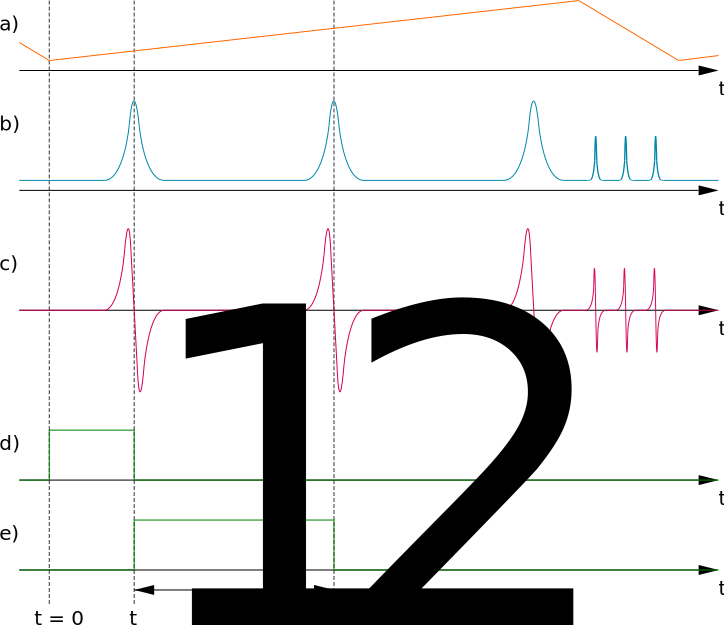
\includegraphics[width=\textwidth-4cm]{gfx/FPI_signal-zeitverlauf}
	}}
	\caption[Zeitlicher Verlauf
	FPI-Transmission]{Zeitlicher Verlauf der
	Transmissionssignale des FPIs. Erklärungenen im Text.}
	\label{fig:FPI_signal-zeitverlauf}
\end{figure}
Um regelmäßig Informationen über die Laserfrequenz zu erhalten, wird der
Piezo-Aktuator des Interferometers periodisch mit einer asymmetrischen
Sägezahnspannung betrieben (Abb. \ref{fig:FPI_signal-zeitverlauf}(a)). Abbildung
\ref{fig:FPI_signal-zeitverlauf} zeigt den zeitlichen Verlauf der Signale eines
Lasers innerhalb einer Periode der Sägezahnspannung. Sowohl für den zu
stabilisierenden Laser als auch für den Referenzlaser wird das zeitliche Transmisionssignal (im
Folgenden \textit{Fringepattern} genannt) mit einer Photodiode bei jeder
steigenden Spannungsflanke aufgenommen (Abb.
\ref{fig:FPI_signal-zeitverlauf}(b)). Der Beginn der steigenden Rampe ist der
Trigger für die Zeitskala. Die Positionen der Peaks (im Folgenden
\textit{Fringes} genannt) enthalten Information über die momentane
Laserfrequenz der zu stabilisierenden Laser. Allerdings können nur relative
Frequenzänderungen zwischen verschiedenen Rampenzyklen und \textbf{keine}
Absolutfrequenzen gemessen werden. Um die Information zu verarbeiten, werden
elektronisch Ableitungen der Signale mit steilen Nulldurchgängen generiert (Abb.
\ref{fig:FPI_signal-zeitverlauf}(c)).\par
Beim Start der Rampe werden die TTL-Signale für die \textit{Offsetfringes} der
beiden Laser auf HIGH ($+5\,$V) gesetzt und damit jeweils ein Counter gestartet.
Wird der erste Fringe eines Lasers anhand des Nulldurchgangs seiner Ableitung
detektiert, so wird sein Offsetfringe-TTL-Signal auf LOW ($0\,$V) gesetzt und der
entsprechende Counter gestoppt, wodurch man die Zeit $t_1$ erhält (Abb.
\ref{fig:FPI_signal-zeitverlauf}(d)). Zeitgleich wird das TTL-Signal des
\textit{Interfringes} auf HIGH gesetzt und ein zweiter Counter gestartet.
Folgt der zweite Fringe des entsprechenden Lasers, wird das
Interfringe-TTL-Signal auf LOW gesetzt und auch der zweite Counter gestoppt,
der die Zeit $t_2-t_1$ liefert (Abb. \ref{fig:FPI_signal-zeitverlauf}(e)). Nach
einer steigenden Flanke erhält man somit die in Tab. \ref{tab:laserzeiten}
aufgelisteten Zeiten.\par
\begin{table}
	%Summe der Breiten muss 0.91 mal \textwidth sein.
	\begin{tabular}{p{0.22\textwidth}p{0.25\textwidth}p{0.44\textwidth}}
		\toprule
		Bezeichung & Zeiten in Abb. \ref{fig:FPI_signal-zeitverlauf} & Beschreibung \\
		\midrule[1px]
		\hline
		$t_{OD}$ & $t_{1,D}$ & Offsetfringe des Diodenlasers \\
		$t_{ID}$ & $t_{2,D}-t_{1,D}$ & Interfringe des Diodenlasers \\
		$t_{OR}$ & $t_{1,R}$ & Offsetfringe des Referenzlasers \\
		$t_{IR}$ & $t_{2,R}-t_{1,R}$ & Interfringe des Referenzlasers \\
		\bottomrule[1px]
	\end{tabular}
	\caption[Fringezeiten]{Zeiten, die nach einer steigenden
	Flanke des Interferometers zur Verfügung stehen.}
	\label{tab:laserzeiten}
\end{table}
Nun drifte der zu stabilisierende Laser ein wenig in der Frequenz und eine
beliebige folgende Rampe liefert die Zeit $t_{OD}'$ und $t_{ID}'$. Die Drift des
Lasers auf der Zeitachse ergibt sich somit zu
\begin{equation}\label{eq:FPI_zeitdrift}
	\Delta T=\left(t_{OD}'-t_{OR}'\right)-\left(t_{OD}-t_{OR}\right)\,.
\end{equation}
Die Zeitdifferenz muss aufgrund der begrenzten Stabilität der Rampe und der
thermischen Drifts des FPIs relativ zum Referenzlaser ausgedrückt werden. Nach
Gl.
\eqref{eq:FPI_zeit-eichung} ergibt sich für den Frequenzdrift
\begin{equation}\label{eq:FPI_frequenzdrift_01}
	\Delta\nu=\frac{4vn_r\text{FSR}}{\lambda}\cdot\Delta T\,.
\end{equation}
Wie schon erwähnt ist die Längenänderung des Resonators zwischen zwei Fringes
genau $\frac{\lambda}{4}$, was zu einer Rampengeschwindigkeit von
$v=\frac{\lambda}{4t_{ID}}$ führt. Insgesamt folgt also für den Frequenzdrift
zwischen erster und beliebiger folgender Rampe
\begin{equation}\label{eq:FPI_frequenzdrift_02}
	\Delta\nu=n_r\text{FSR}\cdot\frac{\left[\left(t_{OD}'-t_{OR}'\right)-\left(t_{OD}-t_{OR}\right)\right]}{t_{ID}}\,.
\end{equation}
Es ist jedoch aus Stabilitätsgründen sicherer, den Interfringe des
Referenz-Lasers zu verwenden, wobei darauf zu achten ist, dass der Interfringe
von der Laserfrequenz abhängt. Daher müssen die Zeiten mit den
Absolutwellenlängen der Laser gewichtet werden:
\begin{equation}\label{eq:FPI_frequenzdrift_03}
	\Delta\nu=n_r\text{FSR}\cdot\frac{\left[\left(t_{OD}'-t_{OR}'\right)-\left(t_{OD}-t_{OR}\right)\right]}{t_{IR}}\cdot\frac{\lambda_R}{\lambda_D}\,.
\end{equation}
Dabei genügt es, die Absolutwellenlängen vor dem Experiment grob mit einem
Wavemeter zu bestimmen. Mit der Annahme einer festen Wellenlänge
des Referenzlasers $\lambda_R$ und einer Absolutwellenlänge
des zu stabilisierenden Lasers von $\lambda_D=(770,0\pm0,1)\,$nm folgt
\begin{equation}\label{eq:FPI_frequenzdrift_fehler}
	\Delta(\Delta\nu)=\Delta\nu\cdot\frac{\Delta\lambda_D}{\lambda_D}\approx1.3\cdot10^{-4}\cdot\Delta\nu\,.
\end{equation}
Für die maximal direkt messbare Relativfrequenz von
$\Delta\nu=\text{FSR}\approx300\,$MHz ergibt sich
$\Delta(\Delta\nu)\approx39\,$kHz. Somit kann mit einer vor
dem Experiment bestimmten Absolutwellenlänge über große Frequenzbereiche hinweg
ohne messbaren Fehler gearbeitet werden.\par
Mithilfe von $\Delta\nu$ kann nun ein Regelkreis betrieben werden, der den zu
stabilisierenden Laser auf eine beliebige Relativfrequenz stabilisiert. Wie
schon erwähnt kann diese Technik benutzt werden, um mehrere Laser
gleichzeitig zu kontrollieren, indem man sie vor dem Interferometer mit dem
Referenzlaser zusammenführt und danach wieder trennt. Die Frequenzkontrolle
ist sehr unempfindlich gegen Drifts. Sowohl thermische Drifts des FSR als auch
Schwankungen des Brechnungsindex $n_r$ sind vernachlässigbar
\cite{kuschnick:2000:diplomarbeit}.\par
Die Technik birgt aber auch Nachteile: Da die Rampenfrequenz wie hier auf etwa
$60\,$Hz begrenzt ist, erhält man nur in Abständen von etwa $17\,$ms
Informationen über die Laser. Zeitlich entsprechend grob ist daher auch die
Regelschleife. Analytische Messungen setzten aus Gründen der Messzeit einen
schnellen Wechsel zwischen den Anregungs- und Ionisationsfrequenzen der verschiedenen
Isotope voraus. Dazu ist es wichtig, die Laserfrequenzen möglichst schnell
und sicher über mehrere GHz zu verstimmen. Um die Laser weiter als einen FSR
verfahren zu können, müssen Sprünge in benachbarte FSR detektiert werden. Dies ist nur möglich, wenn pro Rampe maximal ein halber FSR verfahren wird. Um ein sicheres
Verstimmen der Laser zu gewährleisten, setzt man die Maximalverstimmung pro
Rampe auf $\nicefrac{\text{FSR}}{3}$ fest. Für eine Verstimmung von $10\,$GHz benötigt
man also etwa $1,7\,$s, was für Isotopenverhältnismessungen sehr lange ist.
Daher wird hier eine weitere kommerzielle Stabilisierungstechnik verwendet, die auf einem festen
\textit{Quadraturinterferometer} basiert und im folgenden Abschnitt genauer
beschrieben werden soll.

\section{Quadraturinterferometer}\label{sec:quadraturinterferometer}
Ein festes Interferometer hat gegenüber einem scanning Interferometer den
Vorteil, dass Laserinformationen mit wesentlich höheren Raten erlangt werden
können, da man z.B. im Gegensatz zum obigen Fall nicht durch die Rampenrate
zeitlich limitiert ist. Die einfachste Stabilisierungsmethode im Gegensatz zu
den in Abschn. \ref{sec:haensch-couillaud} und \ref{sec:pound-drever-hall}
vorgestellten Stabilisierungsmethoden mit festem FPI ist es, auf ein Transmissionsmaximum zu
stabilisieren. Ein Problem ist allerdings die nicht eindeutige Richtung, in die
geregelt werde soll. Driftet der Laser vom Transmissionsmaximum weg, hat man
aufgrund der Symmetrie der Airy-Funktion keine Information über die Richtung
der Drift. Es ist jedoch möglich, mit dem Aufbau eines
Quadraturinterferometers die Phase \eqref{eq:FPI_phase}, die unmittelbar von der Frequenz abgängt, absolut zu
bestimmen\footnote{Die absolute Bestimmung gilt natürlich nicht für die
Frequenz, da die Phase FSR-periodisch in der Frequenz ist.}. Im folgenden
Abschnitt soll das Prinzip eines Quadraturinterferometers erklärt und
anschließend die kommerzielle Variante
\textit{iScan$^\text{\textregistered}$} vorgestellt werden
(\cite{kinder:2003:dissertation}, \cite{iscan_hardware_guide}).

\subsection{Prinzip}\label{subsec:quadraturinterferometer_prinzip}
\begin{figure}[h]
 	\centering
 	\fbox{\parbox{\dimexpr \linewidth - 2\fboxrule - 2\fboxsep}{
 	\centering
	    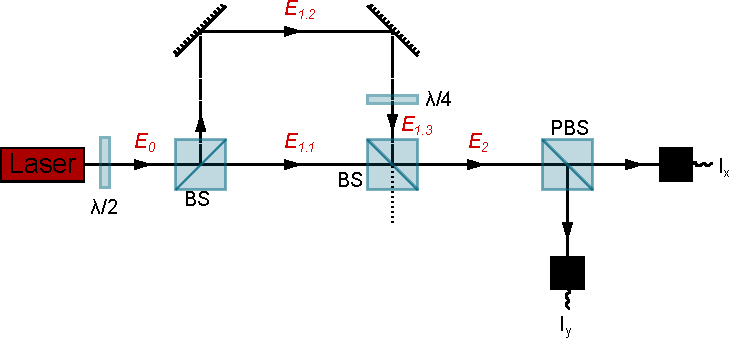
\includegraphics[width=\textwidth-2cm]{gfx/quadraturinterferometer_aufbau}
	}}
	\caption[Quadraturinterferometer - prinzipieller Aufbau]{Prinzipieller Aufbau
	eines Quadraturinterferometers.}
	\label{fig:quadraturinterferometer_aufbau}
\end{figure}
Abbildung \ref{fig:quadraturinterferometer_aufbau} zeigt den prinzipiellen
Aufbau eines festen Quadraturinterferometers. Ein Teil des Strahls des zu stabilisierenden
Lasers wird in den Aufbau eingekoppelt. Das linear polarisierte
Licht des Lasers lässt sich durch die elektrische Feldkomponente
\begin{equation}\label{eq:quadraturinterfferometer_01}
	\vec{E}_0=E_0\left[\cos{(\alpha)}\hat{\vec{e}}_x+\sin{(\alpha)}\hat{\vec{e}}_y\right]\cos{(\omega
	t)}
\end{equation}
beschreiben. Hierbei sind $\hat{\vec{e}}_x$ und $\hat{\vec{e}}_y$ die
Einheitsvektoren der Polarisationskomponenten, wobei $\hat{\vec{e}}_x$ parallel
zur optischen Achse des Aufbaus ist. $\alpha$ ist der Winkel zwischen der
Polarisation des Lasers und der optischen Achse, welche durch die Stellung des
$\nicefrac{\lambda}{4}$-Plättchens definiert ist. Wahlweise kann $\alpha$ durch
ein zusätzliches $\nicefrac{\lambda}{2}$-Plättchen variiert werden.
Der erste 50/50-Strahlteiler teilt den Eingangsstrahl in zwei Strahlen
$\vec{E}_{1.1}$ und $\vec{E}_{1.2}$ der halben Eingangsleistung auf. Dabei erfährt einer der
beiden Strahlen durch eine Verlängerung des optischen Wegs (gestrichelt)
gegenüber dem anderen sog.
Referenzstrahl eine relative Phasenverschiebung $\phi$. Es gilt also
\begin{equation}\label{eq:quadraturinterfferometer_02}
	\begin{split}
		\vec{E}_{1.1}&=\frac{E_0}{\sqrt{2}}\left[\cos{(\alpha)}\hat{\vec{e}}_x+\sin{(\alpha)}\hat{\vec{e}}_y\right]\cos{(\omega
		t)}\\
		\vec{E}_{1.2}&=\frac{E_0}{\sqrt{2}}\left[\cos{(\alpha)}\hat{\vec{e}}_x+\sin{(\alpha)}\hat{\vec{e}}_y\right]\cos{(\omega
		t+\phi)}\,.
	\end{split}
\end{equation}
Zusätzlich werden die Komponten von $\vec{E}_{1.2}$ durch das
$\nicefrac{\lambda}{4}$-Plättchen um $\nicefrac{\pi}{2}$ in der
Phase zueinander verschoben, wodurch elliptisch polarisiertes Licht gemäß
\begin{equation}\label{eq:quadraturinterfferometer_03}
	\vec{E}_{1.3}=\frac{E_0}{\sqrt{2}}\left[\cos{(\alpha)}\cos{(\omega
	t+\phi)}\hat{\vec{e}}_x+\sin{(\alpha)}\sin{(\omega
	t+\phi)}\hat{\vec{e}}_y\right]
\end{equation}
entsteht. Die schnelle Komponente ($\parallel\hat{\vec{e}}_y$) hat also einen
Vorsprung in der Phase von $+\nicefrac{\pi}{2}$ erhalten. Durch einen zweiten
50/50-Strahlteiler werden beide Teilstrahlen $\vec{E}_{1.1}$ und $\vec{E}_{1.3}$
gemischt. Danach erhält man zwei gleiche Strahlen mit dem jeweiligen
elektrischen Feldvektor
\begin{equation}\label{eq:quadraturinterfferometer_04}
	\begin{split}
		\vec{E}_2=\frac{E_0}{2}\Big[&\cos{(\alpha)}\left[\cos{(\omega
		t+\phi)}+\cos{(\omega t)}\right]\hat{\vec{e}}_x\\
		+&\sin{(\alpha)}\left[\sin{(\omega t+\phi)}+\cos{(\omega
		t)}\right]\hat{\vec{e}}_y\Big]\,.
	\end{split}
\end{equation}
Anschließend wird bei einem der Strahlen durch einen
Polarisationsstrahlteiler die Polarisation getrennt und mit Photodioden detektiert. An den Photodioden
entstehen somit die zeitlich gemittelten Ströme
\begin{subequations}\label{eq:quadraturinterfferometer_05}
	\begin{equation}\label{eq:quadraturinterfferometer_05_Ix}
		\begin{split}
			I_x(\alpha,\phi)&=\int\limits_0^{\frac{2\pi}{\omega}}\abs{\frac{E_0}{2}\cos{(\alpha)}\left[\cos{(\omega
			t+\phi)}+\cos{(\omega t)}\right]}^2\dd{t}\\
			&=\frac{E_0^2}{4}\cos^2{(\alpha)}\left[1+\sin{(\phi)}\right]
		\end{split}
	\end{equation}
	\begin{equation}\label{eq:quadraturinterfferometer_05_Iy}
		\begin{split}
			I_y(\alpha,\phi)&=\int\limits_0^{\frac{2\pi}{\omega}}\abs{\frac{E_0}{2}\sin{(\alpha)}\left[\sin{(\omega
			t+\phi)}+\cos{(\omega t)}\right]}^2\dd{t}\\
			&=\frac{E_0^2}{4}\sin^2{(\alpha)}\left[1+\cos{(\phi)}\right]\,,
		\end{split}
	\end{equation}	
\end{subequations}
welche phasenabhängig sind und zwei Quadraturkomponenten wie in
Abb.\ref{fig:quadratursignale} darstellen. Dabei wurde ein $\alpha$ von
$\nicefrac{\pi}{2}$ gewählt, was beide Komponenten gleich stark wichtet. Somit
lässt sich die Phase $\phi$ sehr einfach auf dem Kreis, der zweidimensional in
Quadraturdarstellung entsteht, absolut ablesen.
Eine bestimmte Laserfrequenz entspricht also einem Punkt auf dem Kreis. Es kann also
auf einen bestimmten Kreispunkt und somit auf eine bestimmte Phase bzw. Frequenz
stabilisiert werden. Ein Punkt auf dem Kreis entspricht jedoch unendlich vielen
Frequenzen mit $\nu_0+n\cdot\text{FSR}\,,\,n\in\N$, was demzufolge wieder nur
eine relative Frequenzkontrolle ermöglicht.
\begin{figure}[h]
	\centering
	\footnotesize
	% GNUPLOT: LaTeX picture with Postscript
\begingroup
  \makeatletter
  \providecommand\color[2][]{%
    \GenericError{(gnuplot) \space\space\space\@spaces}{%
      Package color not loaded in conjunction with
      terminal option `colourtext'%
    }{See the gnuplot documentation for explanation.%
    }{Either use 'blacktext' in gnuplot or load the package
      color.sty in LaTeX.}%
    \renewcommand\color[2][]{}%
  }%
  \providecommand\includegraphics[2][]{%
    \GenericError{(gnuplot) \space\space\space\@spaces}{%
      Package graphicx or graphics not loaded%
    }{See the gnuplot documentation for explanation.%
    }{The gnuplot epslatex terminal needs graphicx.sty or graphics.sty.}%
    \renewcommand\includegraphics[2][]{}%
  }%
  \providecommand\rotatebox[2]{#2}%
  \@ifundefined{ifGPcolor}{%
    \newif\ifGPcolor
    \GPcolortrue
  }{}%
  \@ifundefined{ifGPblacktext}{%
    \newif\ifGPblacktext
    \GPblacktexttrue
  }{}%
  % define a \g@addto@macro without @ in the name:
  \let\gplgaddtomacro\g@addto@macro
  % define empty templates for all commands taking text:
  \gdef\gplbacktext{}%
  \gdef\gplfronttext{}%
  \makeatother
  \ifGPblacktext
    % no textcolor at all
    \def\colorrgb#1{}%
    \def\colorgray#1{}%
  \else
    % gray or color?
    \ifGPcolor
      \def\colorrgb#1{\color[rgb]{#1}}%
      \def\colorgray#1{\color[gray]{#1}}%
      \expandafter\def\csname LTw\endcsname{\color{white}}%
      \expandafter\def\csname LTb\endcsname{\color{black}}%
      \expandafter\def\csname LTa\endcsname{\color{black}}%
      \expandafter\def\csname LT0\endcsname{\color[rgb]{1,0,0}}%
      \expandafter\def\csname LT1\endcsname{\color[rgb]{0,1,0}}%
      \expandafter\def\csname LT2\endcsname{\color[rgb]{0,0,1}}%
      \expandafter\def\csname LT3\endcsname{\color[rgb]{1,0,1}}%
      \expandafter\def\csname LT4\endcsname{\color[rgb]{0,1,1}}%
      \expandafter\def\csname LT5\endcsname{\color[rgb]{1,1,0}}%
      \expandafter\def\csname LT6\endcsname{\color[rgb]{0,0,0}}%
      \expandafter\def\csname LT7\endcsname{\color[rgb]{1,0.3,0}}%
      \expandafter\def\csname LT8\endcsname{\color[rgb]{0.5,0.5,0.5}}%
    \else
      % gray
      \def\colorrgb#1{\color{black}}%
      \def\colorgray#1{\color[gray]{#1}}%
      \expandafter\def\csname LTw\endcsname{\color{white}}%
      \expandafter\def\csname LTb\endcsname{\color{black}}%
      \expandafter\def\csname LTa\endcsname{\color{black}}%
      \expandafter\def\csname LT0\endcsname{\color{black}}%
      \expandafter\def\csname LT1\endcsname{\color{black}}%
      \expandafter\def\csname LT2\endcsname{\color{black}}%
      \expandafter\def\csname LT3\endcsname{\color{black}}%
      \expandafter\def\csname LT4\endcsname{\color{black}}%
      \expandafter\def\csname LT5\endcsname{\color{black}}%
      \expandafter\def\csname LT6\endcsname{\color{black}}%
      \expandafter\def\csname LT7\endcsname{\color{black}}%
      \expandafter\def\csname LT8\endcsname{\color{black}}%
    \fi
  \fi
  \setlength{\unitlength}{0.0500bp}%
  \begin{picture}(7200.00,5040.00)%
    \gplgaddtomacro\gplbacktext{%
      \csname LTb\endcsname%
      \put(660,640){\makebox(0,0)[r]{\strut{} 0}}%
      \put(660,1540){\makebox(0,0)[r]{\strut{} 0.1}}%
      \put(660,2441){\makebox(0,0)[r]{\strut{} 0.2}}%
      \put(660,3341){\makebox(0,0)[r]{\strut{} 0.3}}%
      \put(780,440){\makebox(0,0){\strut{} 0}}%
      \put(1215,440){\makebox(0,0){\strut{} 0.5}}%
      \put(1650,440){\makebox(0,0){\strut{} 1}}%
      \put(2084,440){\makebox(0,0){\strut{} 1.5}}%
      \put(2519,440){\makebox(0,0){\strut{} 2}}%
      \put(260,2215){\rotatebox{-270}{\makebox(0,0){\strut{}Intensit{"a}t $\nicefrac{}{E_0^2}$}}}%
      \put(1649,140){\makebox(0,0){\strut{}Phase $\nicefrac{\phi}{\pi}$}}%
    }%
    \gplgaddtomacro\gplfronttext{%
      \csname LTb\endcsname%
      \put(1616,3628){\makebox(0,0)[r]{\strut{}$I_x$}}%
      \csname LTb\endcsname%
      \put(1616,3428){\makebox(0,0)[r]{\strut{}$I_y$}}%
    }%
    \gplgaddtomacro\gplbacktext{%
      \csname LTb\endcsname%
      \put(3553,857){\makebox(0,0)[r]{\strut{} 0}}%
      \csname LTb\endcsname%
      \put(3553,1944){\makebox(0,0)[r]{\strut{} 0.1}}%
      \csname LTb\endcsname%
      \put(3553,3030){\makebox(0,0)[r]{\strut{} 0.2}}%
      \csname LTb\endcsname%
      \put(3890,440){\makebox(0,0){\strut{} 0}}%
      \csname LTb\endcsname%
      \put(4977,440){\makebox(0,0){\strut{} 0.1}}%
      \csname LTb\endcsname%
      \put(6064,440){\makebox(0,0){\strut{} 0.2}}%
      \csname LTb\endcsname%
      \put(3153,2215){\rotatebox{-270}{\makebox(0,0){\strut{}Intensit{"a}t $\nicefrac{I_y}{E_0^2}$}}}%
      \put(5249,140){\makebox(0,0){\strut{}Intensit{"a}t $\nicefrac{I_x}{E_0^2}$}}%
      \csname LTb\endcsname%
      \put(5271,2541){\makebox(0,0)[l]{\strut{}$\phi$}}%
    }%
    \gplgaddtomacro\gplfronttext{%
    }%
    \gplbacktext
    \put(0,0){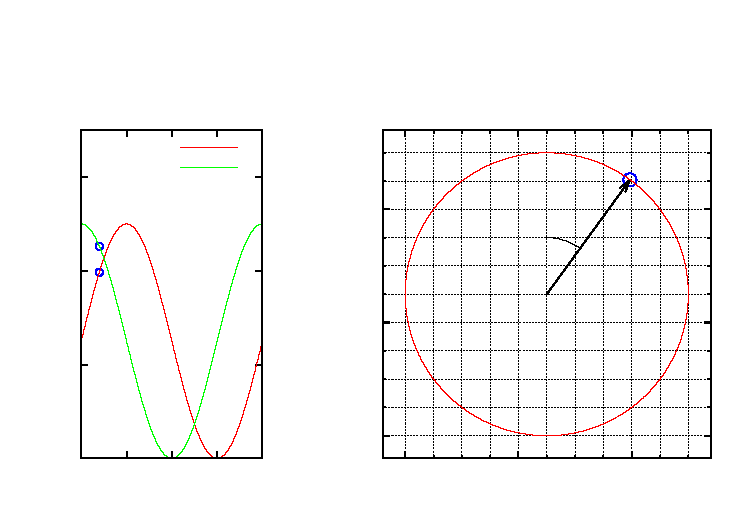
\includegraphics{quadratursignale}}%
    \gplfronttext
  \end{picture}%
\endgroup

	\caption[Quadratursignale]{Photodiodensignale des Quadraturinterferometers
	gemäß Gln. \eqref{eq:quadraturinterfferometer_05} (links) und die
	Quadraturdarstellung (rechts).}
	\label{fig:quadratursignale}
\end{figure}

\subsection{\textit{iScan}$^\text{\textregistered}$}\label{subsec:iScan}
\begin{figure}[h]
 	\centering
 	\fbox{\parbox{\dimexpr \linewidth - 2\fboxrule - 2\fboxsep}{
 	\centering
	    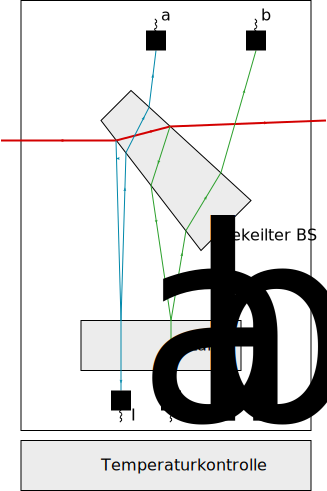
\includegraphics[width=\textwidth-8cm]{gfx/iscan_aufbau}
	}}
	\caption[\textit{iScan head} - Aufbau]{Aufbau
	des \textit{iScan heads} und Strahlengang des zu
	stabilisierenden Lasers.}
	\label{fig:iscan_aufbau}
\end{figure}
Der Aufbau der hier verwendeten kommerziellen Variante eines
Quadraturinterferometers (\textit{iScan head} \cite{iscan_hardware_guide}) ist
in Abb.
\ref{fig:iscan_aufbau} dargestellt. Die Phasenverschiebung
unterscheidet sich beim \textit{iScan} von der oben erklärten Technik insofern,
dass sie nicht durch Polarisationstrennung erzeugt wird, sondern durch
verschiedene optische Weglängen zweier Teilstrahlen, die von einem Etalon
reflektiert werden. Der eingehende rote Strahl ist ein Abgriff des zu
stabilisierenden Lasers. An einem gekeilten Strahlteiler wird dieser in zwei
Teilstrahlen mit unterschiedlicher Phase aufgeteilt (blau und grün dargestellt),
wobei der phasenverschiebende optische Wegunterschied das rote Teilstrück
innerhalb des Strahlteilers ist. Beide Strahlen durchlaufen ein Etalon\footnote{Ein Etalon
ist ein Festkörper, der die gleiche Funktion hat wie ein FPI. Seine Grenzflächen
entsprechen dabei den halbdurchlässigen Spiegeln.} mit sehr geringer Finesse und
einem FSR von ca. $7,8\,$GHz. Ein großer Teil des Lichts transmittiert das
Etalon aufgrund der sehr geringen Finesse praktisch interferenzfrei, womit die
Photodiodenströme $I_a$ und $I_b$ ein Maß für die Leistungen beider Teilstrahlen
(blau und grün) sind. Ebensfalls wegen der geringen Finesse entsprechen die
Fringepattern der reflektierten Strahlen am Etalon einer Sinusfunktion mit
positivem Offset (siehe \ref{fig:airy-funktion}). Wählt man den optischen
Wegunterschied optimalerweise so, dass die Phasendifferenz $\nicefrac{\pi}{2}$
ist, erhält man nach Normierung von $a$ und $b$ durch $I_a$ und $I_b$ für den Quadraturplot
wieder einen Kreis wie in Abb. \ref{fig:quadratursignale}, wenn mit der Phase
bzw. der Laserfrequenz parametrisiert wird. Es ist offensichtlich, dass die Form
des Kreises sehr empfindlich gegenüber der Einkopplung in den \textit{iScan
head} ist, da sich der optische Wegunterschied und somit die Phase zwischen den
Teilstrahlen leicht ändern kann. Dadurch kommt es zu einer elliptischen
Verformung, die allerdings durch Modifizierung der Signale in der sog.
\textit{iScan control unit} \cite{iscan_hardware_guide} ausgeglichen werden
kann. Weiterhin können die Quadratursignale in auf einem Oszilloskop im XY-Modus
betrachtet werden. Wird der Laser schnell in der Frequenz um mindestens einen
FSR des \textit{iScans} moduliert, bildet sich ein Kreis, wie in Abb.
\ref{fig:iscan_oszilloskop_bild_01} dargestellt. Kommt es währenddessen zu
Modensprüngen, springt auch der Punkt des Kreisbogens und es ergibt sich ein
Signal wie in Abb. \ref{fig:iscan_oszilloskop_bild_02}. Starke
Leistungsschwankungen des Lasers, die durch das Feed-Forward verursacht werden,
führen zu Änderungen des Kreisradius, was prinzipiell keine negativen Einflüsse
auf die Messung bzw. Stabilisierung hat
(Abb. \ref{fig:iscan_oszilloskop_bild_03}).
Die Elektronik dieser \textit{iScan control unit} zur analogen Verarbeitung der Signale und zur Laserstabilisierung soll in Kapitel \ref{kap:experimenteller_aufbau} näher betrachtet werden.
Selbstverständlich kann im Gegensatz zum FOL nur ein Laser pro
\textit{iScan}-System stabilisert werden.
%TODO: Fotos Quadraturkreis, Multimode, etc.

\section{Regeltechnik}\label{sec:regeltechnik}
\begin{figure}[h]
 	\centering
 	\fbox{\parbox{\dimexpr \linewidth - 2\fboxrule - 2\fboxsep}{
 	\centering
	    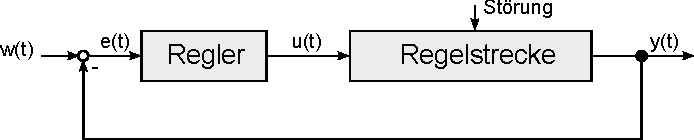
\includegraphics[width=\textwidth-2cm]{gfx/regelkreis}
	}}
	\caption[Regelkreis]{Allgemeiner Regelkreis mit
	negativer Rückkopplung. Erklärungen im Text.}
	\label{fig:regelkreis}
\end{figure}
Bisher wurden nur verschiedene Techniken zur Detektion der
Ist-Frequenz bzw. der Frequenzabweichung zur Sollfrequenz vorgestellt.
In diesem Abschnitt soll die Regeltechnik, die die Laserparameter zum Erreichen
der Soll-Frequenz manipuliert, vorgestellt werden. Der Ablauf eines
einfachen Standardregelkreises ist in Abb. \ref{fig:regelkreis} dargestellt. Am
Eingang liegt der Sollwert (\textit{Führungsgröße} genannt) $w(t)$ an. Die
Differenz zum Istwert bzw. zur \textit{Regelgröße} $y(t)$ ist die
\textit{Regelabweichung} $e(t)=w(t)-y(t)$. Der \textit{Regler} berechnet die
\textit{Stellgröße} $u(t)$, also den Parameter des Systems, der die Regelgröße
über die \textit{Regelstrecke} manipuliert. Dabei besteht die Regelstrecke aus
allen gewollten frequenzbeeinflussenden Komponenten des Lasersystems. Die
Regelstrecke wird dabei von äußeren Einflüssen gestört, was eine Regelung
überhaupt erst nötig macht. Im Falle des FOL kann $w(t)$ eine
gewünschte Relativfrequenz und $y(t)$ die Ist-Relativfrequenz gemäß Gl.
\eqref{eq:FPI_frequenzdrift_03} sein. Im Falle der \textit{iScan}-Regelung sind
$w(t)$ und $y(t)$ die normierten Soll- und Ist-Spannungen der Quadratursignale. $u(t)$
kann ein korrigierendes Offset für die aktuelle Piezospannung bzw. für den über
Feed-Forward linear gekoppelten Strom des Lasers sein.\par
Kern der Regeltechnik ist der Regler, für den verschiedene \textit{Regelglieder}
realisiert und bedarfsweise auch kombiniert werden können.
Dabei unterscheiden sich hier die technischen Realisierungen zwischen
FOL und \textit{iScan} stark voneinander. Die \textit{iScan
control unit} regelt kontinuierlich, was elektronisch und analog umgesetzt
wird. Der Regler des FOLs arbeitet über einen Rechner digital mit zeitlich
quantisierten Regelwerten. Beide Varianten sollen hier kurz erläutert
werden.\par
\begin{figure}[h]
 	\centering
 	\fbox{\parbox{\dimexpr \linewidth - 2\fboxrule - 2\fboxsep}{
		\subfloat[]{
			\label{subfig:operationsverstaerker}
	    	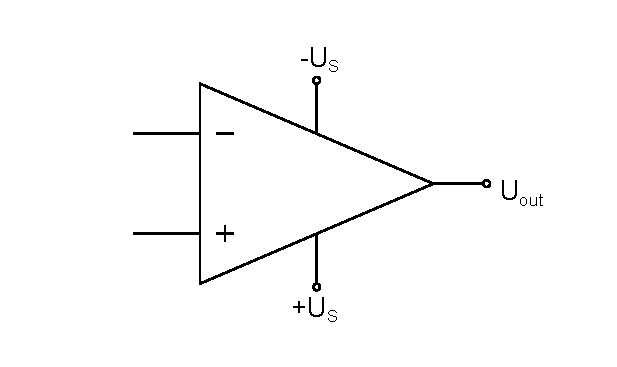
\includegraphics[width=(\textwidth-1cm)/2]{gfx/operationsverstaerker}
	  	}
		\subfloat[]{
			\label{subfig:operationsverstaerker_p-regler}
	    	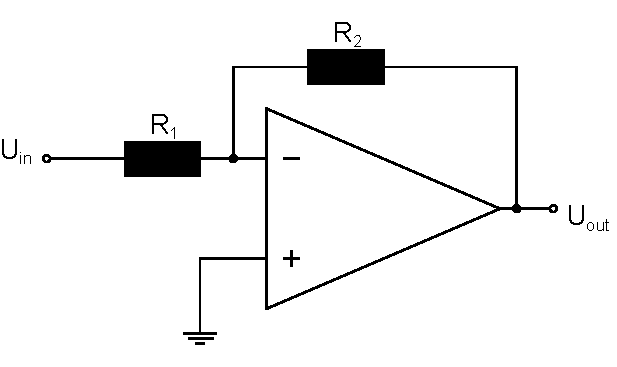
\includegraphics[width=(\textwidth-1cm)/2]{gfx/operationsverstaerker_p-regler}
	  	}\\
	  	\subfloat[]{
			\label{subfig:operationsverstaerker_i-regler}
	    	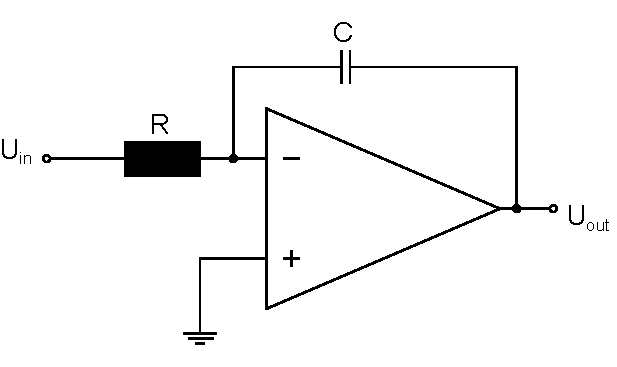
\includegraphics[width=(\textwidth-1cm)/2]{gfx/operationsverstaerker_i-regler}
	    	}
		\subfloat[]{
			\label{subfig:operationsverstaerker_d-regler}
	    	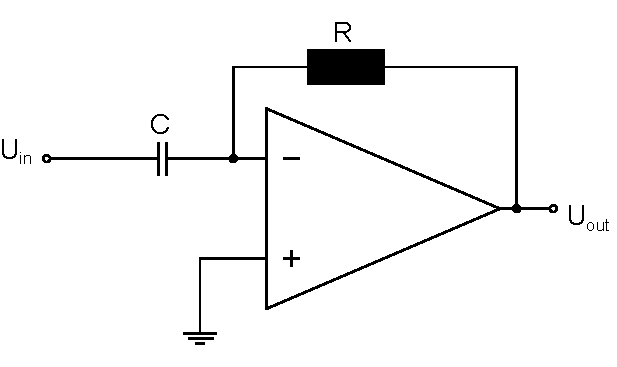
\includegraphics[width=(\textwidth-1cm)/2]{gfx/operationsverstaerker_d-regler}
	    	}
	}}
	\caption[Operationsverstärker, Regler]{(a) zeigt einen Operationsverstärker
	mit invertierendem (-) und nicht-invertierendem
	Eingang (+), Versorgungsspannung $\pm U_S$ und
	Ausgansspannung $U_{out}$. (b), (c) und (d) zeigen die Schaltungen von
	P-, I- und D-Regler mithilfe eines
	Operationsverstärkers.}
	\label{fig:operationsverstaerker}
\end{figure}
Ein kontinuierlicher Regler baut auf einem Operationsverstärker (OP) auf (siehe
\ref{fig:operationsverstaerker}\subref{subfig:operationsverstaerker}). Dieser
hat einen invertierenden (-) und einen nicht-invertierenden (+) Eingang, deren Potentialdifferenz durch die
Versorgungsspannung $\pm U_S$ zu $U_{out}$ verstärkt wird. Durch eine
Rückkopplung der Ausgangsspannung an einen der Eingangskanäle erhält der OP erst
seine Nützlichkeit und verhält sich nach folgenden Regeln:
\begin{enumerate}
       \item Die Potenzialdifferenz zwischen den Eingängen ist null.
       \item Der Stromfluss am Eingang ist nahezu null.
\end{enumerate}
Ein Regler kann aus einem Regelglied oder mehreren Regelgliedern bestehen, wobei
die Grundarten \textit{\textbf{P}roportional-Glied}, \textit{\textbf{I}ntegral-Glied} und
\textit{\textbf{D}ifferenzier-Glied} sind. Im Folgenden ist der Eingang des
jeweiligen Regelglieds die Regelabweichung $e$ bzw. Eingangsspannung $U_{in}$
und der Ausgang die Stellgröße $u$ bzw. Ausgangsspannung $U_{out}$. Dabei muss
zwischen kontinuierlichen und nicht-kontinuierlichen Reglern unterschieden
werden. Ein kontinuierlicher Regler regelt rein elektronisch und weist keine
diskrete Regelzyklen auf. Ein nicht-kontinuierlicher Regler regelt iterativ in
diskreten Regelzyklen $i$.

\subsection{P-Regler}\label{p-regler}
Das Ausgangssignal eines P-Reglers ist proportional zum Eingangssignal:
\begin{equation}\label{eq:p-regler_01}
	u(t)=K_P\cdot e(t)\,,
\end{equation}
wobei $K_P$ die Verstärkung ist. Abbildung
\ref{fig:operationsverstaerker}\subref{subfig:operationsverstaerker_p-regler}
zeigt die Umsetzung für einen kontinuierlichen Regler. Nach Regel 1 liegen die Eingänge des OPs auf Masse und die gesamte Spannung $U_{in}$ fällt an $R_1$ ab.
Ebenso fällt die gesamte Spannung $U_{out}$ an $R_2$ ab, woraus für den
Verstärkungsfaktor
\begin{equation}\label{eq:p-regler_02}
	K_P=-\frac{R_2}{R_1}
\end{equation}
folgt. Beim nicht-kontinuierlichen Regler wird
\begin{equation}\label{eq:p-regler_03}
	u_i=K_P\cdot e_i
\end{equation}
berechnet, wobei der Index $i$ die momentane Iteration bezeichnet und $K_P$ ein
einstellbarer Parameter ist. Ein reiner P-Regler kompensiert zwar schnell die
Abweichung zum Sollwert eines Systems, kann diesen aber nie exakt erreichen, da
sich bei nicht divergierender Einstellung die Regelgröße immer asymptotisch
dem Sollwert nähert und ggf. um diesen alterniert.

\subsection{I-Regler}\label{i-regler}
Das Ausgangssignal des integralwirkenden Reglers, kurz I-Regler, ist
proportional zum über die Zeit integrierten Eingangssignal:
\begin{equation}\label{eq:i-regler_01}
	u(t)=K_I\int\limits_0^te(t')\dd{t'}\,.
\end{equation}
Wichtig ist hierbei, dass es zu keinem Offset im Eingangssignal kommen darf. Ein
kontinuierlicher I-Regler unterscheidet sich gegenüber dem P-Regler dadurch, dass $R_2$ durch eine
Kapazität $C$ ersetzt wird wie in Abb.
\ref{fig:operationsverstaerker}\subref{subfig:operationsverstaerker_i-regler}
dargestellt. Damit gilt
\begin{equation}\label{eq:i-regler_02}
	\begin{split}
		I_{in}&=\frac{U_{in}}{R}=-\fracd{Q}{t}=-C\fracd{}{t}U_{out}\\
		&\Rightarrow\\
		U_{out}(t)&=K_I\int\limits_0^tU_{in}(t')\dd{t'}
		\quad\text{mit}\quad
		K_I=-\frac{1}{RC}\,.
	\end{split}
\end{equation}
Für einen nicht-kontinuierlichen I-Regler ergibt sich
\begin{equation}\label{eq:i-regler_03}
	\begin{split}
		u_i&=K_I\cdot e_i\cdot (t_i-t_{i-1})+u_{i-1}\\
		\text{mit}\quad
		u_{0}&=0\,.
	\end{split}
\end{equation}
Die aktuelle Stellgröße eines I-Reglers ist also abhängig von vergangenen
Stellgrößen. Dies verursacht immer ein Schwingen um den Sollwert, was die
Regelung langsam macht, aber den Vorteil birgt, dass der Sollwert erreicht
werden kann. In paralleler Kombination mit einem P-Regler kommt es bei richtig
eingestellten Verstärkungsfaktoren zu einem Einschwingen auf den Sollwert.

\subsection{D-Regler}\label{d-regler}
Ein D-Regler erzeugt ein Ausgangssignal, das proportional zur zeitlichen
Ableitung des Eingangssignals ist:
\begin{equation}\label{eq:d-regler_01}
	u(t)=K_D\fracd{}{t}e(t)\,.
\end{equation}
Der kontinuierliche D-Regler wird im Gegensatz zum I-Regler durch Tauschen von
Kapazität und Widerstand realisiert, wie Abb.
\ref{fig:operationsverstaerker}\subref{subfig:operationsverstaerker_d-regler}
zeigt. Der durch eine sich zeitlich ändernde Eingangsspannung $U_{in}$ verursachte Strom
\begin{equation}\label{eq:d-regler_02}
	I_{in}=C\fracd{}{t}U_{in}
\end{equation}
muss wegen Regel 2 über den Widerstand $R$ fließen. Da die Spannung, die an $R$
abfällt wegen Regel 1 wieder $U_{out}$ sein muss, folgt hieraus
\begin{equation}\label{eq:d-regler_03}
	\begin{split}
		U_{aus}=K_D\fracd{}{t}U_{in}
		\quad\text{mit}\quad
		K_D=-RC\,.
	\end{split}
\end{equation}
Ein digitaler nicht-kontinuierlicher D-Regler errechnet die Stellgröße über
\begin{equation}\label{eq:i-regler_03}
	\begin{split}
		u_i&=K_D\cdot\frac{e_{i-1}-e_i}{t_{i-1}-t_i}\\
		\text{mit}\quad
		u_{0}&=0\,.
	\end{split}
\end{equation}
Für die meisten Fälle ist eine PI-Regler-Kombination völlig ausreichend.
%TODO: Bild PID-Regler Verhalten, Simulation

\section{Kombination von \textit{iScan} und
FOL}\label{sec:iscan_und_fringe-offset-locking}
Die beiden Stabilisierungstechniken FOL und \textit{iScan} haben
Vor- und Nachteile, von denen letztere im Rahmen dieser Arbeit gegenseitig
kompensiert werden sollen.
Wegen ihrer kontinuierlichen Frequenzkontrolle ist die Regelung der
\textit{iScans} sehr schnell. Sollfrequenzen stellen sich bei optimal
eingestelltem Regler innerhalb von $1$-$2\,$ms ein. Auch große gewünschte
Frequenzverstimmungen von mehreren GHz, wie sie z.B. bei
Isotopenverhältnismessungen nötig sind, können innerhalb weniger Millisekunden
erreicht werden. Damit bietet das \textit{iScan} einen großen Vorteil gegenüber
dem FOL, das zeitlich durch seine Rampenfrequenz und die digitale Verarbeitung
der Frequenzinformationen limitiert ist.
Entscheidender Nachteil des \textit{iScans} ist die starke Anfälligkeit für
Drifts.
Langzeitfrequenzdrifts können mit FOL kompensiert werden, da
diese Methode wie schon erwähnt dank des absolut stabilen He:Ne-Lasers resistent
gegen Drifts ist. Dazu wird die Frequenz mit beiden Techniken parallel
kontrolliert, wobei beide Regelkreise miteinander gekoppelt werden, aber
dabei unabhängig voneinander arbeiten können.\par
Abbildung \ref{fig:regelkreis_kopplung} zeigt schematisch die Kopplung beider
Regelkreise. Der Nutzer kann eine Relativfrequenz zu einer vorher festgelegten
Referenz als Sollwert vorgeben. Die in Abschn. \ref{sec:fringe-offset-locking} erklärte Technik ermittelt die Ist-Relativfrequenz. Die Abweichung zum Sollwert
wird mithilfe des FOL-Reglers mittels Modifizierung des
Sollwerts der \textit{iScan}-Reglung $\nu_{Soll,iScan}$ minimiert. Unabhängig
davon und etwa drei Größenordnungen schneller regelt die \textit{iScan}-Technik
den Laser auf den regelmäßig erneuerten \textit{iScan}-Sollwert
$\nu_{Soll,iScan}$. Sie regelt auf normierte Sollwerte $A$ und $B$ der Photodioden aus Abschn. \ref{subsec:iScan},
welche über eine sog. \textit{Lookup-Table} (LUT) ermittelt werden. Die
LUT ist digital in der \textit{iScan control unit} hinterlegt und mit
Abgleichbeziehungen zwischen den Phasen der Quadraturkreispunkte (s. Abb.
\ref{fig:quadratursignale}) und den Werten von $A$ und $B$ für die tatsächlichen
Relativfrequenzen gefüllt.
Zu stabilisierender Laser und \textit{iScan head} stellen die Regelstrecke der
\textit{iScan}-Stabilisierung dar. Die Regelstrecke des FOLs
umschließt die komplette \textit{iScan}-Stabilisierung.\par
\begin{figure}[h]
 	\centering
 	\fbox{\parbox{\dimexpr \linewidth - 2\fboxrule - 2\fboxsep}{
 	\centering
	    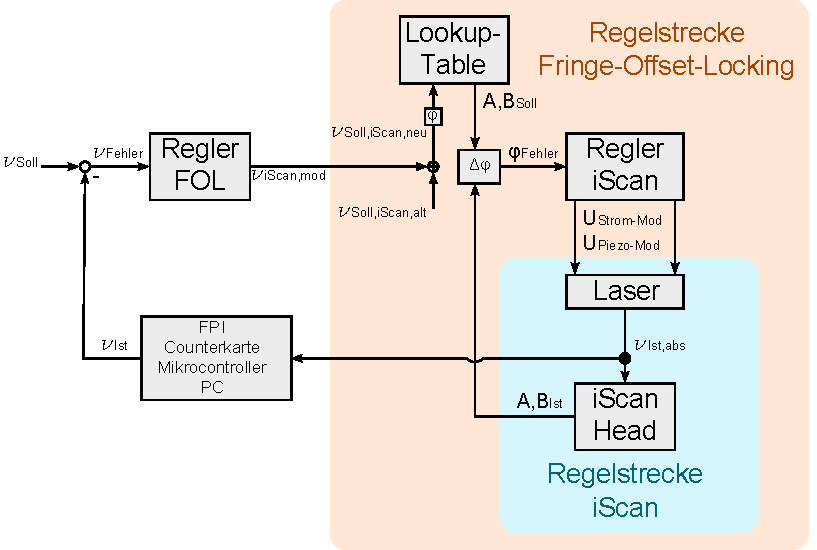
\includegraphics[width=\textwidth-0.5cm]{gfx/regelkreis_kopplung}
	}}
	\caption[Regelkreis - Kopplung]{Kopplung der Regelkreise beider
	Laserstabilisierungstechniken \textit{iScan} und
	FOL. Alle angegebenen Frequenzen außer $\nu_{Ist,abs}$ sind
	Relativfrequenzen relativ zu der jeweiligen
	Referenz der Techniken. Weitere Erklärungen im Text.}
	\label{fig:regelkreis_kopplung}
\end{figure}
Neben den Langzeitdrifts des \textit{iScans} kommt es weiterhin noch zu
einer Verschlechterung der Linearität in der Skalierung des
Phasenquadraturkreises.
Um dies zu kompensieren, wird die LUT mit ihren Abgleichwerten zur
Verfügung gestellt, wobei es nötig ist, diese regelmäßig zu erneuern.
Darüber hinaus muss auch der digital hinterlegte FSR des \textit{iScans} mit dem
aktuellen, tatsächlichen FSR abgeglichen werden. Nur so ist eine lineare
Skalierung mit dem richtigen Proportionalitätsfaktor zwischen Phase und
Relativfrequenz möglich. Umgesetzt wird der Abgleich, indem mittels eines
\textit{Lock-In-Verstärkers}
\textit{LaseLock$^\text{\textregistered}$}\footnote{Für eine nähere Beschreibung
des Geräts sei auf das Handbuch verwiesen.} der Firma \textit{TEM} \cite{laselock} das FPI auf einen Transmissionsfringe des He:Ne-Lasers festgehalten und gleichzeitig durch Verfahren der Frequenz des Lasers des entsprechenden \textit{iScans} ein Transmissionsfringepattern
aufgenommen wird. Dabei wird die Frequenz gemäß der aktuellen LUT verfahren. Bei
perfektem Nichtlinearitätsausgleich der LUT, also bei perfekt linearem
Verfahren der Laserfrequenz, wären alle Fringes äquidistant mit einem Abstand
von einem FSR des FPIs in der Skala des \textit{iScans}. Aus der Abweichung von
diesem Idealfall lässt sich sowohl eine Korrektur für die LUT als auch der tatsächliche
FSR des \textit{iScans} berechnen. Die softwareseitige Realisierung wird in Kap.
\ref{kap:software} beschrieben.\par
Wie sich in Kap. \ref{kap:charakterisierung} zeigen wird, ist eine perfekte
Linearisierung der \textit{iScans} nicht möglich, woraus für das Anfahren großer
Relativfrequenzen inakzeptable Fehler resultieren. Diese Abweichung zu den
tatsächlichen Sollfrequenzen kann wiederum durch Nachregeln mit der
FOL-Technik ausgeglichen werden.\par
Mit der Kombination der beiden Stabilisierungstechniken wird also ein sowohl
lang- als auch kurzzeitstabiles Lasersystem erwartet, mit dem darüber hinaus große, schnelle und sichere Frequenzverstimmungen möglich sind.
Detailbeschreibungen für die hard- und softwareseitige Implementierung folgen in
Kap. \ref{kap:experimenteller_aufbau} und \ref{kap:software}.